%\documentclass[conference,compsoc]{IEEEtran}
\documentclass[letterpaper,twocolumn,10pt]{article}
\usepackage{usenix}

%%%%%%%%%%%%%%%%%%%%%%%%%%%%%%%%%%%%%%%%%%%%%%%%%%%%%%%%%%%%%%%%%%%%%%%%%%%%%%%%
% CUSTOM PACKAGES
%%%%%%%%%%%%%%%%%%%%%%%%%%%%%%%%%%%%%%%%%%%%%%%%%%%%%%%%%%%%%%%%%%%%%%%%%%%%%%%%
\usepackage{tikz}
\usetikzlibrary{patterns.meta,backgrounds, calc, arrows.meta, intersections, patterns, positioning, shapes.misc, fadings, through,decorations.pathreplacing,shapes}
\usepackage{amsmath}
\usepackage{enumitem}
\usepackage{csquotes}
\usepackage{dashrule}
\usepackage{amssymb}
\usepackage[normalem]{ulem} % for \dashuline
\usepackage[ruled,vlined]{algorithm2e}
\usepackage{listofitems}
\usepackage{xspace}
\usepackage{pgfplots}
\usepackage{makecell}
\usepackage{adjustbox}
\usepackage{minted}
\usepackage{acronym}
\usepackage{subcaption}
\usepackage{hyperref}
% \usepackage{dingbat}
\usepackage{pifont}
\usepackage{amssymb}
\usepackage{censor}
\usepackage{booktabs}
\usepackage{float}
\usepackage{tcolorbox}
\usepackage{listings}
\usepackage{pifont}
\newcommand{\cmark}{\ding{51}}%
\newcommand{\xmark}{\ding{55}}%
\usepackage[capitalise,nameinlink,noabbrev,english]{cleveref}
% thousand separator
\usepackage[english]{babel}
\usepackage{numprint}
\npthousandsep{,}
\pagestyle{empty}
\providecommand*{\listingautorefname}{Listing}
\renewcommand{\sectionautorefname}{Section}
\renewcommand{\subsectionautorefname}{Section}
\renewcommand{\subsubsectionautorefname}{Section}
%\renewcommand{\listingautorefname}{Listing}

\makeatletter
\let\old@lstKV@SwitchCases\lstKV@SwitchCases
\def\lstKV@SwitchCases#1#2#3{}
\makeatother
\usepackage{lstlinebgrd}
\makeatletter
\let\lstKV@SwitchCases\old@lstKV@SwitchCases

\lst@Key{numbers}{none}{%
    \def\lst@PlaceNumber{\lst@linebgrd}%
    \lstKV@SwitchCases{#1}%
    {none:\\%
     left:\def\lst@PlaceNumber{\llap{\normalfont
                \lst@numberstyle{\thelstnumber}\kern\lst@numbersep}\lst@linebgrd}\\%
     right:\def\lst@PlaceNumber{\rlap{\normalfont
                \kern\linewidth \kern\lst@numbersep
                \lst@numberstyle{\thelstnumber}}\lst@linebgrd}%
    }{\PackageError{Listings}{Numbers #1 unknown}\@ehc}}
\makeatother


% minted configuration
\setminted[c]{ %
    linenos=true,             % Line numbers
    numbersep=2pt,
    autogobble=true,          % Automatically remove common white space
    framesep=2mm,
    fontsize=\scriptsize,
    xleftmargin=2mm,
    tabsize=2,
}


\usepackage{filecontents}

%%%%%%%%%%%%%%%%%%%%%%%%%%%%%%%%%%%%%%%%%%%%%%%%%%%%%%%%%%%%%%%%%%%%%%%%%%%%%%%%
% COMMENTING SETUP
%%%%%%%%%%%%%%%%%%%%%%%%%%%%%%%%%%%%%%%%%%%%%%%%%%%%%%%%%%%%%%%%%%%%%%%%%%%%%%%%

% Enable or disable reviews
\newif\ifreview
%\reviewtrue
\reviewfalse

\definecolor{amber}{rgb}{1.0, 0.75, 0.0}
\newcounter{ReviewerID}
\readlist*\annotationcolors{blue, red, orange, green, purple, amber, brown, olive}
\newcommand{\newreviewer}[2]{%
        \ifnum \theReviewerID=\annotationcolorslen
        \setcounter{ReviewerID}{0} % cycle through colors
        \fi
        \stepcounter{ReviewerID}%
        \expandafter\edef\csname bootstrap#1\endcsname{%
                \expandafter\def\csname #1\endcsname####1{%
                        \ifreview%
                         {\noexpand\color{\annotationcolors[\theReviewerID]} {\noexpand\bf{\noexpand\fbox{#2}} {\noexpand\it ####1} }}
                        \else%
                         {}% disable annotations
                        \fi%
                }%
        }%
        \csname bootstrap#1\endcsname%
}

% List of reviewers
% Command: \newreviewer{latexcommand}{visiblename}
% You will be able to use a command \latexcommand{comment}
% to generate a colored comment prepended by visiblename.
\newreviewer{mao}{mao}
\newreviewer{ed}{ed}
\newreviewer{mat}{mat}
\newreviewer{mb}{mb} % marcel
\newreviewer{yiwen}{yiwen}

\DeclareRobustCommand{\encircle}[1]{%
  \tikz[baseline=(X.base)] 
    \node (X) [draw, shape=circle, inner sep=0em,text width=1em, text centered] {\scriptsize #1};}


%%%%%%%%%%%%%%%%%%%%%%%%%%%%%%%%%%%%%%%%%%%%%%%%%%%%%%%%%%%%%%%%%%%%%%%%%%%%%%%%
% MACROS
%%%%%%%%%%%%%%%%%%%%%%%%%%%%%%%%%%%%%%%%%%%%%%%%%%%%%%%%%%%%%%%%%%%%%%%%%%%%%%%%

%\newcommand{\sysname}{SHMUZZli\xspace}
\newcommand{\sysname}{ScHMuzz\xspace}
\newcommand{\taemu}{TÄMU\xspace}
\newcommand{\stageone}{Exploration\xspace}
\newcommand{\stagetwo}{Double Fetch Snapshot Fuzzing\xspace}
\newcommand{\stagethree}{Distillation\xspace}
\newcommand{\mitee}{MiTEE\xspace}
\newcommand{\teegris}{TEEGris\xspace}
\newcommand{\optee}{OP-TEE\xspace}
\newcommand{\tsix}{T6\xspace}
\newcommand{\beanpod}{Beanpod\xspace}
\newcommand{\kinibi}{Kinibi\xspace}
\newcommand{\qsee}{QSEE\xspace}
\newcommand{\opensource}{\url{https://anonymous.4open.science/r/ta-df-78EB}\xspace}

% dataset
\newcommand{\nummiteeTAs}{12\xspace}
\newcommand{\nummiteeTAsharnessed}{10\xspace}
\newcommand{\numbeanpodTAs}{11\xspace}
\newcommand{\numbeanpodTAsharnessed}{5\xspace}
\newcommand{\numteegrisTAs}{33\xspace}
\newcommand{\numteegrisTAsharnessed}{9\xspace}
\newcommand{\numqseeTAs}{4\xspace}
\newcommand{\numqseeTAsharnessed}{3\xspace}
\newcommand{\numkinibiTAs}{6\xspace}
\newcommand{\numkinibiTAsharnessed}{3\xspace}
\newcommand{\numTAs}{66\xspace}
\newcommand{\numTAsharnessed}{30\xspace}
\newcommand{\numTEEs}{five\xspace}

% fuzzing campaign
\newcommand{\numruns}{five\xspace}
\newcommand{\numTAsdfqsee}{2\xspace}
\newcommand{\numTAsdfteegris}{7\xspace}
\newcommand{\numTAsdfmitee}{8\xspace}
\newcommand{\numTAsdfkinibi}{2\xspace}
\newcommand{\numTAsdfbeanpod}{4\xspace}
\newcommand{\numTAsdf}{23\xspace}

\newcommand{\numdfsqsee}{866,145\xspace}
\newcommand{\numdfsteegris}{33\xspace}
\newcommand{\numdfsmitee}{41,918\xspace}
\newcommand{\numdfskinibi}{3,301\xspace}
\newcommand{\numdfsbeanpod}{1,852\xspace}
\newcommand{\numdfs}{913,249\xspace}

\newcommand{\numdfsmergeqsee}{1,670\xspace}
\newcommand{\numdfsmergeteegris}{33\xspace}
\newcommand{\numdfsmergemitee}{10,469\xspace}
\newcommand{\numdfsmergekinibi}{3,256\xspace}
\newcommand{\numdfsmergebeanpod}{1,804\xspace}
\newcommand{\numdfsmerge}{17,232\xspace}

\newcommand{\numcrashesqsee}{6\xspace}
\newcommand{\numcrashesteegris}{32\xspace}
\newcommand{\numcrashesmitee}{44\xspace}
\newcommand{\numcrasheskinibi}{123\xspace}
\newcommand{\numcrashesbeanpod}{125\xspace}
\newcommand{\numcrashes}{330\xspace}


\newcommand{\numcrashesdistillqsee}{6\xspace}
\newcommand{\numcrashesdistillteegris}{32\xspace}
\newcommand{\numcrashesdistillmitee}{8\xspace}
\newcommand{\numcrashesdistillkinibi}{7\xspace}
\newcommand{\numcrashesdistillbeanpod}{9\xspace}
\newcommand{\numcrashesdistill}{62\xspace}

\newcommand{\numvulns}{six\xspace}
\newcommand{\numvulnsrepro}{five\xspace}
\newcommand{\numvulnTAs}{five\xspace}
\newcommand{\numvulnTEEs}{five\xspace}

% df harnesses
%\newcommand{\eighteigthce}{88ce8e6b-8646-4092-bb78faf5b55ff4df\xspace}
%\newcommand{\aseventhreefour}{a734eed9-d6a1-4244-aa507c99719e7b7f\xspace}
%\newcommand{\sixfivefivea}{655a4b46-cd77-11ea-aafbf382a6988e7b\xspace}
%\newcommand{\eightaaa}{8aaaf201-2460-0000-7143fe4f7c823c80\xspace}
%\newcommand{\zeroeightzeroone}{08010203000000000000000000000000\xspace}
%\newcommand{\onefourbzero}{14b0aad8-c011-4a3f-b66aca8d0e66f273\xspace}
%\newcommand{\dfonee}{df1edda8627911e980ae507b9d9a7e7d\xspace}
%\newcommand{\fivethreefourfive}{00000000-0000-0000-0000-53454d655345\xspace}
%\newcommand{\anineeightfive}{a985d3eb-3b52-4d44-be6c-628a813561e8\xspace}
%\newcommand{\foureightfourfour}{00000000-0000-0000-0000-000048444350\xspace}
%\newcommand{\foursixsixtwo}{00000000-0000-0000-0000-4662436b6d52\xspace}
%\newcommand{\threesevensevene}{377ee4e8-af0e-474f-a9d636a9268fe85c\xspace}
%\newcommand{\threedzeroeight}{3d08821c-33a6-11e6-a1fa089e01c83aa2\xspace}

\newcommand{\eighteigthce}{Mlipay\xspace}
\newcommand{\aseventhreefour}{GF\_TA\xspace}
\newcommand{\sixfivefivea}{OTrPAPP\xspace}
\newcommand{\eightaaa}{Mirisikm\xspace}
\newcommand{\zeroeightzeroone}{ifaa-key\xspace}
\newcommand{\onefourbzero}{fido\xspace}
\newcommand{\dfonee}{paytrigger\xspace}
\newcommand{\fivethreefourfive}{SEMeSE\xspace}
\newcommand{\anineeightfive}{eID\xspace}
\newcommand{\foureightfourfour}{HDCP\xspace}
\newcommand{\foursixsixtwo}{FbCkmR\xspace}
\newcommand{\threesevensevene}{SoterApp\xspace}
\newcommand{\threedzeroeight}{VSIMApp\xspace}


% reshaping comparison


\newcommand{\numexecseighteightce}{490'558\xspace}
\newcommand{\numexecsdfeighteightce}{75'528\xspace}
\newcommand{\numexecsdfperceighteightce}{15\%\xspace}

\newcommand{\numexecsaseventhreefour}{14'741'203\xspace}
\newcommand{\numexecsdfaseventhreefour}{2'757'134\xspace}
\newcommand{\numexecsdfpercaseventhreefour}{18\%\xspace}

\newcommand{\numexecssixfivefivea}{6'718'937\xspace}
\newcommand{\numexecsdfsixfivefivea}{39'572\xspace}
\newcommand{\numexecsdfpercsixfivefivea}{0.5\%\xspace}

\newcommand{\numexecseightaaa}{75'843\xspace}
\newcommand{\numexecsdfeightaaa}{53'027\xspace}
\newcommand{\numexecsdfperceightaaa}{69\%\xspace}

\newcommand{\numexecszeroeightzeroone}{32'143'889\xspace}
\newcommand{\numexecsdfzeroeightzeroone}{2'480'790\xspace}
\newcommand{\numexecsdfperczeroeightzeroone}{7\%\xspace}

\newcommand{\numexecsonefourbzero}{11'938\xspace}
\newcommand{\numexecsdfonefourbzero}{866\xspace}
\newcommand{\numexecsdfperconefourbzero}{7\%\xspace}

\newcommand{\numexecsdfonee}{812'135\xspace}
\newcommand{\numexecsdfdfonee}{41'193\xspace}
\newcommand{\numexecsdfpercdfonee}{5\%\xspace}

\newcommand{\numexecsfivethreefourfive}{24'364\xspace}
\newcommand{\numexecsdffivethreefourfive}{22260\xspace}
\newcommand{\numexecsdfpercfivethreefourfive}{91\%\xspace}

\newcommand{\numexecsanineeightfive}{19'345\xspace}
\newcommand{\numexecsdfanineeightfive}{5215\xspace}
\newcommand{\numexecsdfpercanineeightfive}{27\%\xspace}

\newcommand{\numexecsfoureightfourfour}{52'012\xspace}
\newcommand{\numexecsdffoureightfourfour}{891\xspace}
\newcommand{\numexecsdfpercfoureightfourfour}{1\%\xspace}

\newcommand{\numexecsthreedzeroeight}{3'863'250\xspace}
\newcommand{\numexecsdfthreedzeroeight}{117'860\xspace}
\newcommand{\numexecsdfpercthreedzeroeight}{3\%\xspace}

\newcommand{\numexecsfoursixsixtwo}{568'237\xspace}
\newcommand{\numexecsdffoursixsixtwo}{127'009\xspace}
\newcommand{\numexecsdfpercfoursixsixtwo}{15\%\xspace}

\newcommand{\numexecsthreesevensevene}{1'788'240\xspace}
\newcommand{\numexecsdfthreesevensevene}{1'041'636\xspace}
\newcommand{\numexecsdfpercthreesevensevene}{58\%\xspace}

\newcommand{\numexecs}{61'309'951\xspace}
\newcommand{\numexecsdf}{6'762'981\xspace}
\newcommand{\numexecsdfperc}{11\%\xspace}

% Rust TAs
\newcommand{\numRustTAs}{28\xspace}
\newcommand{\numRustTAsShm}{6\xspace}
\newcommand{\numRustTAsnoShm}{22\xspace}

%%%%%%%%%%%%%%%%%%%%%%%%%%%%%%%%%%%%%%%%%%%%%%%%%%%%%%%%%%%%%%%%%%%%%%%%%%%%%%%%
\begin{document}
%%%%%%%%%%%%%%%%%%%%%%%%%%%%%%%%%%%%%%%%%%%%%%%%%%%%%%%%%%%%%%%%%%%%%%%%%%%%%%%%

%don't want date printed
\date{}

\title{\Large \bf Oversharing: Exposing Double Fetch Vulnerabilities in Trusted Applications} 

\author
{Authors Anonymized
} % end author

%\author{
%{\rm Philipp Mao} \hspace{.5em}
%{\rm Yiwen Xu} \hspace{.5em}
%{\rm Mathias Payer} \\
%{\rm Marcel Busch} \hspace{.5em}
%EPFL, Lausanne, Switzerland
%} % end author

\maketitle

%%%%%%%%%%%%%%%%%%%%%%%%%%%%%%%%%%%%%%%%%%%%%%%%%%%%%%%%%%%%%%%%%%%%%%%%%%%%%%%%
\begin{abstract}

Modern Android smartphones leverage a Trusted Execution Environment (TEE) to 
protect security-critical services. Trusted Applications (TAs) run in the TEE and 
communicate with the untrusted normal world.
To meet performance requirements, normal world clients may share physical memory pages with 
TAs. While efficient, this design introduces the risk of double fetches, 
in which a malicious normal world attacker can modify shared memory between multiple accesses 
by a TA, potentially leading to time-of-check-to-time-of-use (TOCTTOU) vulnerabilities.

We present the first study of shared memory double fetch vulnerabilities in TAs. 
To automatically detect attacker-triggerable TOCTTOU  
vulnerabilities in binary-only TAs, we present \sysname, a novel three-stage oracle for such vulnerabilities 
leveraging coverage-guided fuzzing.
We evaluate \sysname on \numTAsharnessed{} TAs, uncovering \numvulns{} 
0-day TOCTTOU vulnerabilities in \numvulnTAs{} TAs across all major commercial TEEs. We reproduce 
our findings on commercial phones, demonstrating for the first time the wide use of zero-copy 
shared memory in commercial TEEs. Looking to the future, we find that even TAs 
written in memory-safe languages are affected by shared memory double fetches. 
Given that both existing and future TAs are affected by shared memory double fetches, we 
propose a mitigation that makes shared memory, a performance optimization, explicitly opt-in. Our mitigation 
prevents all discovered double fetch vulnerabilities from being exploited without 
changes to the existing TAs. 
This work addresses a critical and previously overlooked fault line, shared memory, 
affecting TAs deployed on billions of devices.

\end{abstract}
%%%%%%%%%%%%%%%%%%%%%%%%%%%%%%%%%%%%%%%%%%%%%%%%%%%%%%%%%%%%%%%%%%%%%%%%%%%%%%%%

%%%%%%%%%%%%%%%%%%%%%%%%%%%%%%%%%%%%%%%%%%%%%%%%%%%%%%%%%%%%%%%%%%%%%%%%%%%%%%%%
\section{Introduction}\label{sec:introduction}
%%%%%%%%%%%%%%%%%%%%%%%%%%%%%%%%%%%%%%%%%%%%%%%%%%%%%%%%%%%%%%%%%%%%%%%%%%%%%%%%

Trusted Execution Environments (TEEs) form the last line of defense on modern Android devices, protecting 
sensitive data even against a compromised normal world. The normal world 
runs the Android user space and the Linux kernel.  
To interact with the TEE, the normal world communicates with 
Trusted Applications (TAs). Each TA implements a subset of the functionality 
required to interact with TEE-protected data, such as biometrics, DRM, or digital payments. Bugs in TAs 
are critical as they allow normal world-based attackers to gain a foothold in the TEE~\cite{beniaini2017trustissues,berard2018kinibi,busch2020finding,rollback,globalconfusion,Komaromy2021UnboxYourPhone,Li2024DiveIntoAndroidTA,AdamskiGuilbonPeterlin2019SamsungTrustZone,Makkaveev2019TrustZoneFuzzing,AdamTC}.

The GlobalPlatform API is a set of specifications that were introduced to 
give TA developers a standardized interface and enable TAs to be deployed on 
different GlobalPlatform-compliant TEEs. The specification is now widely adopted by all  
relevant TEE implementations~\cite{globalconfusion}. GlobalPlatform specifies how a normal 
world client application (NWCA) exchanges data with a TA. The NWCA can send input either as a value (an 
integer) or a memory buffer. This memory buffer may be shared between the 
normal and secure worlds. \textit{Shared} in this case means the NWCA and the TA are both 
accessing the same physical memory page when accessing the input buffer. Such zero-copy 
shared memory is crucial for performance-critical TA use-cases such as DRM.

Unfortunately, while shared memory is great for performance, handling shared 
memory securely is difficult due to double fetches. Double fetches arise when 
a value is fetched from the same offset in the shared memory twice by the TA. 
Since the memory may be shared with the untrusted NWCA, a malicious NWCA may intentionally 
modify the value between the fetches. 
In the worst case, this allows the malicious NWCA to trigger time-of-check-to-time-of-use (TOCTTOU) 
vulnerabilities, which may be exploited to compromise the TA.
%\mb{emphasize the attacker model. We're dealing with a maliciously acting NWCA intending to systematically abuse double fetches with an impact on security. These double fetches would never be a problem if it was not for the very precise exploitation of race conditions carried out by untrusted, malicous NWCAs}. 

Prior work on TA security has extensively examined vulnerabilities arising from 
the absence of rollback protection~\cite{rollback}, flawed API design~\cite{globalconfusion}, 
and improper handling of untrusted data~\cite{AdamskiGuilbonPeterlin2019SamsungTrustZone,teezz,trustdies}. 
Separately, prior work on automatic double fetch vulnerability detection has focused on kernels 
or enclaves with source-code access~\cite{decaf,deadline,wang2017double,chen2024enclavefuzz}, 
and does not transfer to proprietary, binary-only TAs. 
As a result, vulnerabilities arising from shared memory handling in TAs have remained unexplored.

\ed{Nice!}
This gap persists due to two fundamental challenges. \textbf{First}, there is no oracle for
automatically detecting double fetch vulnerabilities in proprietary, binary-only TAs.
\textbf{Second}, the lack of such a detection capability has prevented a systematic study of
whether proprietary commercial TEEs actually support zero-copy shared memory. 

To close this gap, we propose \sysname, a three-stage oracle to 
automatically detect TOCTTOU vulnerabilities in proprietary binary-only targets. 
\sysname leverages coverage-guided fuzzing in an emulator to explore the target and 
discover inputs that trigger overlapped fetches from shared memory. \sysname creates 
a snapshot just before the second fetch, which, after deduplication, results in a 
snapshot for each uniquely discovered double fetch location in the target.
Leveraging \stagetwo, \sysname determines if a given overlapped fetch leads 
to a vulnerability by fuzzing the double-fetched value. 
Finally, \sysname filters the crashes found during \stagetwo 
for crashes which are only triggerable due to shared memory double fetches, i.e., true 
TOCTTOU vulnerabilities. \sysname automatically 
and precisely detects TOCTTOU vulnerabilities and works for binary-only 
targets.

We implement \sysname for GlobalPlatform-compliant TAs. We create a representative dataset consisting of 
\numTAs{} up-to-date TAs from \numTEEs{} TEEs, deployed on Commercial-Off-The-Shelf (COTS) phones. 
We then apply \sysname to the \numTAsharnessed{} TAs, which operate directly on shared memory (instead of 
operating on a local copy).
In total, \sysname detected \numdfsmerge{} overlapped fetches in \numTAsdf TAs across \textbf{all major} TEEs. 
Furthermore, \sysname detected 
\numvulns{} TOCTTOU vulnerabilities in \numvulnTAs{} TAs, leading to memory corruptions such as 
stack-based overflows or double frees in TAs from \qsee, \teegris, and \mitee. 
Leveraging the corpus of discovered double fetches, we conduct the first systematic study of 
zero-copy shared memory support across commercial TEEs. 
We demonstrate that four out of five major TEEs support zero-copy shared memory.
We reproduce the discovered double fetch vulnerabilities on our COTS testing devices. 
We have responsibly disclosed all discovered vulnerabilities to the affected vendors.

All TAs in our dataset are written in memory-unsafe languages (C/C++). 
However, there is a push in the TEE space for TAs written in memory-safe languages such as 
Rust~\cite{rustee,teaclave}. Applying \sysname to these TAs, we find that even TAs written 
in Rust operate on shared memory and discuss how shared memory breaks Rust's safety guarantees.

Our findings demonstrate that double fetches due to shared memory are an important 
security issue for TAs (both commercially deployed TAs and future TAs written in Rust). 
We hypothesize that the root cause of the vulnerabilities we discovered is the 
TA developers' unawareness of zero-copy shared memory. 
We propose an extension to the GlobalPlatform specification that requires explicit opt-in for 
zero-copy shared memory. Our mitigation successfully fixes the vulnerabilities found by \sysname, 
without requiring modifications of the affected TAs. We demonstrate the feasibility of our mitigation 
by extending \optee, the de facto TEE reference implementation. We are in discussion 
with the GlobalPlatform consortium to amend the specification with our extension.
In summary, we make the following contributions:

\begin{itemize}
    \item Identifying the attack surface of shared memory double fetches for TAs.
    \item Designing and implementing \sysname, an oracle to automatically detect TOCTTOU vulnerabilities 
    in binary-only targets, leveraging dynamic analysis.
    \item Applying \sysname to a representative corpus of COTS TAs and demonstrating both \sysname's capabilities 
    and the widespread impact of TOCTTOU vulnerabilities.
    \item Demonstrating that even TAs written in a memory-safe language are affected by shared memory 
    double fetches.
    \item Proposing an extension to the GlobalPlatform specification, which makes shared memory 
    opt-in, mitigating all detected vulnerabilities.
\end{itemize}

Our implementation of \sysname and our mitigation is open source and available at \opensource.

%%%%%%%%%%%%%%%%%%%%%%%%%%%%%%%%%%%%%%%%%%%%%%%%%%%%%%%%%%%%%%%%%%%%%%%%%%%%%%%%
\section{Background}\label{sec:background}
%%%%%%%%%%%%%%%%%%%%%%%%%%%%%%%%%%%%%%%%%%%%%%%%%%%%%%%%%%%%%%%%%%%%%%%%%%%%%%%%

\begin{listing}[]
    \input{listings/ta.tex}                                                                                                                     \captionof{lstlisting}{
       A TA's \texttt{TA\_InvokeCommandEntryPoint} function. The TA expects a single
       argument buffer, containing an \texttt{in\_data} structure. While executing this function, the TA operates directly on the shared memory 
        (\texttt{params[0].memref.buffer}) and ends up having three overlapped fetches.
       The first fetch is marked in \colorbox{blue!40}{blue} and the second fetches are marked in \colorbox{red!40}{red}.
       While the double fetch on line 21 is harmless, the double fetch on line 23 may lead to a heap buffer overflow if 
       a malicious NWCA modifies the value of \texttt{in->size} between lines 16 and 23. The code path of the double 
       fetch on line 24 leads to a null pointer dereference, however this bug is triggerable without shared memory 
        double fetches.
    }
    \label{lst:exdf}
\end{listing}

\begin{figure}[h]
  \centering
  \centering
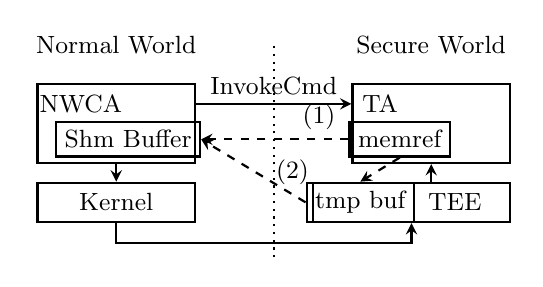
\begin{tikzpicture}%[every node/.style={font=\fontfamily{lmvtt}\selectfont\footnotesize}]
    \small
    \coordinate (normal) at (-2,0);
    \coordinate (secure) at (2,0);

%\node[draw, minimum width=5cm, minimum height=0.5cm, thick] (sm) at (0,-0.75) {Secure Monitor};
        
\begin{scope}[shift=(normal)]
    \coordinate (capos) at (0,1);
    \coordinate (kernelpos) at (0,0);
    \node at (0,2) {Normal World};    
    \node[draw, minimum width=2cm, minimum height=1cm, thick] (ca) at (capos) {};
    \node[draw, minimum width=2cm, minimum height=0.5cm, thick] (kernel) at (kernelpos) {Kernel};
    \begin{scope}[shift=(capos)]
        \node[draw, minimum width=0cm, minimum height=0cm, thick] (shm) at (0.15,-0.2) {Shm Buffer};
        %\node[draw, dashed, fill=blue!20, minimum width=2.5cm, minimum height=0.5cm, thick] (copen) at (0,0.6) {\scriptsize \texttt{OpenSession}};
    \end{scope}
    \node[align=center] at ($(capos.north) + (-0.45cm,0.25cm)$) {NWCA};
\end{scope}

\begin{scope}[shift=(secure)]
    \coordinate (tapos) at (0,1);
    \coordinate (teepos) at (-0.25,0);
    \node at (0,2) {Secure World};    
    \node[draw, minimum width=2cm, minimum height=1cm, thick] (ta) at (tapos) {};
    \node[draw, minimum width=2.5cm, minimum height=0.5cm, thick] (tee) at (teepos) {};
    \begin{scope}[shift=(tapos)]
        \node[draw, minimum width=0cm, minimum height=0cm, thick] (memref) at (-0.4,-0.2) {memref};
    \end{scope}
    \begin{scope}[shift=(teepos)]
        \node[draw, minimum width=0cm, minimum height=0cm, thick] (tmpshm) at (-0.65,-0) {tmp buf};
    \end{scope}
    \node[align=center] at ($(teepos.north) + (0.55cm,0cm)$) {TEE};

\end{scope}
    \node[align=center] at ($(tapos.north) + (-0.65cm,0.25cm)$) {TA};

\draw[->, thick, >=stealth] ($(ca.east) + (0,0.25)$) -- ($(ta.west) + (0,0.25)$) node[midway, above, sloped] {\small{InvokeCmd}};
\draw[->, thick, dashed, >=stealth] ($(memref.west) + (0,0)$) -- ($(shm.east) + (0,0)$) node[pos=0.2, above, sloped] {(1)};
\draw[->, thick, dashed, >=stealth] ($(tmpshm.west) + (0,0)$) -- ($(shm.east) + (0,0)$) node[pos=0.125, above] {(2)};
\draw[->, thick, dashed, >=stealth] ($(memref.south) + (0,0)$) -- ($(tmpshm.north) + (0,0)$) node[midway, above, sloped] {};

\draw[->, thick, >=stealth] ($(ca.south) + (0,0)$) -- ($(kernel.north) + (0,0)$) node[midway, above, sloped] {};
\draw[->, thick, >=stealth] 
    ($(kernel.south) + (0,0)$) 
    -- ($(kernel.south) + (0,-0.25)$)
    -- ($(tee.south) + (0,-0.25)$)
    -- ($(tee.south) + (0,0)$);
    
%\draw[->, thick, >=stealth] ($(kernel.south) + (0,0)$) -- ($(sm.north) + (-2,0)$) node[midway, above, sloped] {};
%\draw[->, thick, >=stealth] ($(sm.north) + (2,0)$) -- ($(tee.south) + (0.25,0)$) node[midway, above, sloped] {};
\draw[->, thick, >=stealth] ($(tee.north) + (0.25,0)$) -- ($(ta.south) + (0,0)$) node[midway, above, sloped] {};

\draw[-, thick, dotted] (0,-0.7) -- (0,2);
%\node at (0.4,1.75) {Secure World};    

%\draw[->, thick, >=stealth] (copen.east) -- (create.west) node[midway, above, sloped] {};
%\draw[->, thick, >=stealth] (copen.east) -- (open.west) node[midway, above, sloped] {};
%\draw[->, thick, >=stealth] (cinvok.east) -- (invoke.west) node[midway, above, sloped] {};
%\draw[->, thick, >=stealth] (cclose.east) -- (close.west) node[midway, above, sloped] {};
%\draw[->, thick, >=stealth] (cclose.east) -- (destroy.west) node[midway, above, sloped] {};
%
%%\draw[<->, thick, >=stealth] ($(gpapi.east) + (0,0.)$) -- ($(tee.west) + (0,0)$) node[midway, above, sloped] {};
%\draw[<->, thick, >=stealth] (ta.east) -- (tee.west) node[midway, above, sloped] {\footnotesize libc API};
%\draw[<->, thick, >=stealth] ($(ta.east) + (0,-0.75)$) -- ($(tee.west) + (0,-0.75)$) node[midway, above, sloped] {\footnotesize TEE API};


\end{tikzpicture}



  %\includegraphics[width=0.4\textwidth]{figures/GlobalPlatformOverview.png}
  \caption{
    An overview of how shared memory facilitates communication between a NWCA and a TA.
    In scenario (1), double fetch vulnerabilities are possible, as the \texttt{memref} 
    buffer pointer of the TA points to the physical page of the buffer in the NWCA. 
    In scenario (2), the TEE makes a local copy of the buffer, and the TA's \texttt{memref} buffer 
    points to that local copy.
    }
  \label{fig:shmex}
\end{figure}

\begin{figure}[]
  \centering
  \centering
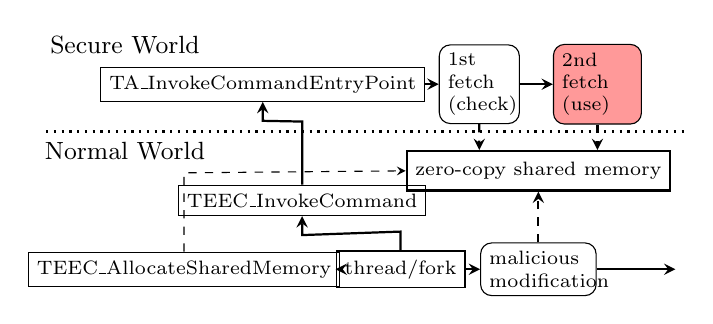
\begin{tikzpicture}%[every node/.style={font=\fontfamily{lmvtt}\selectfont\footnotesize}]
    \small
    \coordinate (normal) at (0,-1);
    \coordinate (secure) at (0,0.6);

\begin{scope}[shift=(normal)]
    \node at (-3.25,0.75) {Normal World};    
    \node[draw] (allocshm) at (-2.5,-0.75) {\scriptsize TEEC\_AllocateSharedMemory};
    \node[draw] (fork) at (0.25,-0.75) {\scriptsize{thread/fork}};
    \node[draw] (cinvoke) at (-1,0.125) {\scriptsize TEEC\_InvokeCommand};
    \node[draw, align=center, rounded corners] (mod) at (2,-0.75) {\scriptsize \parbox{1.25cm}{malicious\\modification}};
    \node[draw, minimum width=3cm, minimum height=0.5cm, thick] (shm) at (2,0.5) {\scriptsize{zero-copy shared memory}};
\end{scope}

\begin{scope}[shift=(secure)]
    \node at (-3.25,0.5) {Secure World};    
    \node[draw] (invoke) at (-1.5,0) {\scriptsize{TA\_InvokeCommandEntryPoint}};
    \node[draw, align=center, rounded corners] (check) at (1.25,0) {\scriptsize\parbox{0.8cm}{1st fetch\\(check)}};
    \node[draw, align=center, fill=red!40, rounded corners] (use) at (2.75,0) {\scriptsize\parbox{0.9cm}{2nd fetch\\(use)}};
\end{scope}

\draw[-, thick, dotted] (-4.25,0) -- (3.85,0);
%\node at (0.4,1.75) {Secure World};    

\draw[->, thick, >=stealth] (allocshm.east) -- (fork.west) node[midway, above, sloped] {};
\draw[->, thick, >=stealth] (fork.east) -- (mod.west) node[midway, above, sloped] {};
\draw[->, thick, >=stealth] (mod.east) -- ($(mod.east) + (1,0)$) node[midway, above, sloped] {};
\draw[->, thick, >=stealth] (invoke.east) -- (check.west) node[midway, above, sloped] {};
\draw[->, thick, >=stealth] (check.east) -- (use.west) node[midway, above, sloped] {};

\draw[->, dashed, thick, >=stealth] (mod.north) -- ($(shm.south) + (0,0)$) node[midway, above, sloped] {};
\draw[->, dashed, thick, >=stealth] (check.south) -- ($(shm.north) + (-0.75,0)$) node[midway, above, sloped] {};
\draw[->, dashed, thick, >=stealth] (use.south) -- ($(shm.north) + (0.75,0)$) node[midway, above, sloped] {};

\draw[->, thick, >=stealth]
    ($(fork.north) + (0,0)$)
    -- ($(fork.north) + (0,0.24)$)
    -- ($(cinvoke.south) + (0,-0.24)$)
    -- ($(cinvoke.south)$);

\draw[->, thick, >=stealth]
    ($(cinvoke.north) + (0,0)$)
    -- ($(cinvoke.north) + (0,0.8)$)
    -- ($(invoke.south) + (0,-0.24)$)
    -- ($(invoke.south)$);

\draw[->, dashed, >=stealth]
    ($(allocshm.north) + (0,0)$)
    -- ($(allocshm.north) + (0,1)$)
    -- ($(shm.west) + (0,0)$);



%\draw[->, thick, >=stealth] (copen.east) -- (open.west) node[midway, above, sloped] {};
%\draw[->, thick, >=stealth] (cinvok.east) -- (invoke.west) node[midway, above, sloped] {};
%\draw[->, thick, >=stealth] (cclose.east) -- (close.west) node[midway, above, sloped] {};
%\draw[->, thick, >=stealth] (cclose.east) -- (destroy.west) node[midway, above, sloped] {};
%
%%\draw[<->, thick, >=stealth] ($(gpapi.east) + (0,0.)$) -- ($(tee.west) + (0,0)$) node[midway, above, sloped] {};
%\draw[<->, thick, >=stealth] (ta.east) -- (tee.west) node[midway, above, sloped] {\footnotesize libc API};
%\draw[<->, thick, >=stealth] ($(ta.east) + (0,-0.75)$) -- ($(tee.west) + (0,-0.75)$) node[midway, above, sloped] {\footnotesize TEE API};


\end{tikzpicture}



  \caption{
    TOCTTOU attack on zero-copy shared memory between the normal and secure world.
    \texttt{TEEC\_AllocateSharedMemory} and \texttt{TEEC\_InvokeCommand} are part of the GlobalPlatform 
    API used by the NWCA to communicate with the TEE/TA.
    }
  \label{fig:tocttouex}
\end{figure}

TEEs deployed on modern Android smartphones are based on ARM TrustZone. 
TrustZone enables hardware-enforced partitioning of the execution context into 
the secure world and the normal world. Code running in the normal world does not 
have access to the memory of the secure world. Only code signed by the phone 
vendor runs in the secure world. Code running in the secure world is referred 
to as the TEE, comprised of TAs and the TEE OS. TAs are user space applications, 
each of which encapsulates a specific TEE use-case, such as DRM, digital 
payments, or biometrics.

NWCAs communicate with TAs to access TEE functionality. Nowadays, most NWCAs and TAs 
leverage the GlobalPlatform APIs, a set of standardized API specifications that enable 
interoperability for NWCAs/TAs between different TEE implementations. The logical 
channel defined by the GlobalPlatform API allows a NWCA to call a command handling 
function (\texttt{TA\_InvokeCommandEntryPoint}) in the TA.  
The arguments passed by the NWCA to this function include the \texttt{commandID}, specifying 
which command is invoked, \texttt{param\_types}, specifying the parameter types, 
and an array of up to four parameters, \texttt{params}. 
Each parameter may either be a \texttt{value} (two 32-bit integers) or a 
\texttt{memref} (a pointer to a memory buffer and its size). 
\autoref{lst:exdf} shows a TA's \texttt{TA\_InvokeCommandEntryPoint} function.
The TA retrieves the input buffer from the NWCA on Line 13.

To pass data from the normal to the secure world, physical pages are shared 
between the normal and secure world, henceforth referred to as shared memory. 
When the NWCA invokes the command handler of a TA with a \texttt{memref} 
parameter, the kernel driver forwards the physical addresses of the NWCA-allocated 
memory buffer to the TEE, which itself maps these physical pages to access the data 
from the normal world. The TEE implementation may map 
the physical pages directly into the TA's address space, or it may first copy
the contents of the NWCA's memory buffer to a temporary buffer. In the first case, the 
pointer in any given \texttt{memref} parameter points to memory that is shared 
with the NWCA. As a consequence, modifications of the buffer contents by the NWCA, 
during the execution of \texttt{TA\_InvokeCommandEntryPoint}, are also visible to the 
TA in the secure world. \autoref{fig:shmex} gives an overview of how the TEE may pass 
memory buffers from the NWCA to the TA's \texttt{memref} buffer.

We refer to the definitions of \textsc{DEADLINE}~\cite{deadline} for double fetches.
The precondition for \textbf{double fetch vulnerabilities} is an \textbf{overlapped fetch}, where data 
is read from the same shared memory range after the range has been previously read/written to. 
An overlapped fetch itself may not lead to a security violation. There needs to be a \textbf{relation}
between the shared memory regions accessed by the two fetches. If the value of the second fetch 
destroys this relation due to changes between fetches, it leads to \textbf{double fetch bugs}.  
These double fetch bugs may turn into security vulnerabilities depending on the context of the 
double fetch. A canonical example is a TOCTTOU vulnerability, where the target program uses the 
first fetch to validate a value in shared memory and the second fetch to subsequently use that value. 
\autoref{fig:tocttouex} shows how a malicious NWCA triggers such a TOCTTOU vulnerability in a TA. 

\begin{figure*}[h!]
  \centering
  \input{figures/overview.tex}
  \caption{
    Overview of \sysname and its three phases. To analyze a TA, \sysname requires the TA binary itself and a fuzzing harness. In the \stageone phase, the TA is fuzzed with the harness. Snapshots are created after observing an overlapped fetch. These snapshots are passed to \stagetwo, where the TA state is restored just before the second fetch and the value fetched from memory is fuzzed. All resulting crashes 
    are then passed to \stagethree, where \sysname determines if a crash is only triggerable due to shared memory double fetches.
    }
  \label{fig:overview}
\end{figure*}

The TA in \autoref{lst:exdf} has three overlapped fetches (we assume the value of \texttt{in->size} is fetched from memory 
on every access). The overlapped
fetch when handling command 1, on Line 21, while technically a double fetch bug due to breaking the relation 
between the check and print, is not a memory safety violation, as the second value is simply 
used for logging. However, the overlapped fetch when handling command 2 is a TOCTTOU vulnerability, as the 
second fetched value is used as the size in the \texttt{memcpy} operation. The size checks and allocations are done on the 
stale value retrieved with the first fetch, while the \texttt{memcpy} operation uses the second fetched 
value, which may have been changed between Lines 16 and 23 to a value larger than 
the first fetch, leading to a heap buffer overflow. The overlapped fetch on Line 24 is not a 
double fetch bug, but still leads to a crash. We discuss how \sysname distinguishes between 
these three cases in \autoref{sec:design}.

As illustrated by the TA in \autoref{lst:exdf}, TOCTTOU vulnerabilities may lead to memory 
corruption. Memory corruption vulnerabilities in TAs are extremely interesting 
to attackers as they may be exploited from the normal world to achieve code execution 
in the vulnerable TA~\cite{fiasccco,beniaini2017trustissues,berard2018kinibi,busch2020finding,rollback,globalconfusion,Komaromy2021UnboxYourPhone,Li2024DiveIntoAndroidTA,AdamskiGuilbonPeterlin2019SamsungTrustZone,Makkaveev2019TrustZoneFuzzing,AdamTC}, allowing the attacker to pivot to the secure world.
Furthermore, while in other contexts, access to shared memory is made explicit to 
the developer, such as \texttt{copy\_from\_user} in the Linux kernel, in the TA 
context, there is no such mechanism, and it is up to the TA developer to securely  
handle the \texttt{memref} buffer pointer. 

%%%%%%%%%%%%%%%%%%%%%%%%%%%%%%%%%%%%%%%%%%%%%%%%%%%%%%%%%%%%%%%%%%%%%%%%%%%%%%%%
\section{Design}\label{sec:design} 
%%%%%%%%%%%%%%%%%%%%%%%%%%%%%%%%%%%%%%%%%%%%%%%%%%%%%%%%%%%%%%%%%%%%%%%%%%%%%%%%


% challenge analyze large dataset of binary-only TAs and find attacker triggerable df vulns automatically
% dynamic approach: 1) reproducible double fetch vulns from clearly defined GlobalPlatform entrypoint
% dynamic approach: 2) bochspwn demonstrates emulation + shm tracing to detect overlapped fetches in binary-only target
% problem of dynamic approach is target coverage (bochspwn just runs target normally): 
% STAGE 1, EXPLORATION: use coverage-guided fuzzing to explore target and detect overlapped fetches
% bochspwn leaves analysis of overlapped fetch -> df bug to manual triage
% deadline detects bug but analysis of bug -> vuln is manual
% manual triage infeasible (nr of fetches + reverse engineering effort)
% dynamic fuzzing approaches are unable to precisely target a given df 
% STAGE 2, DF FUZZING: snapshot fuzzing of double fetched value
% prior dynamic fuzzing approaches can not automatically distinguish if crash is due to df or could be triggered normally
% STAGE 3, DISTILLATION: replay of df input + crash, without shm modification to check for crash

We observe the absence of an oracle for shared memory TOCTTOU vulnerabilities in TAs.
Although TOCTTOU vulnerabilities may lead to critical memory corruption vulnerabilities, due to the 
absence of such an oracle, this attack surface went unnoticed.
To address this challenge, we introduce \sysname, a novel three-stage oracle  
for automatic TOCTTOU vulnerability detection in binary-only TAs. 
Leveraging \sysname we present the first ecosystem-wide study of TOCTTOU vulnerabilities in TAs.

\sysname is based on dynamic analysis. While static analysis 
can, in principle, cover an entire program, it produces a large number of false positives: detected double fetches 
may not be triggerable in practice due to complex path constraints, limited attacker control, or execution 
contexts that are unreachable from the normal world. Such findings are of little security relevance, 
particularly for TAs, where attacker interaction is restricted to a small, well-defined attack surface.
Instead, we deliberately choose a tight under-approximation by leveraging dynamic analysis starting from 
TA entrypoints that are reachable by a NWCA. Furthermore, static analysis for closed-source targets is more 
complex due to decompilation and might suffer from incomplete/incorrect results.

\sysname works in three stages.
1) \textbf{\stageone}: Identify overlapped fetches in attacker-reachable code. 2) \textbf{\stagetwo}: Determine 
whether a given double fetched value leads to a vulnerability. 3) \textbf{\stagethree}: Determine whether 
a discovered vulnerability is \emph{only} triggerable with shared-memory double fetching.
Each stage addresses a distinct limitation of prior work. \autoref{fig:overview} gives an overview of \sysname 
and its three stages.

\subsection{\stageone}

In the \stageone phase, the target program is fuzzed in an emulated environment, 
and accesses to shared memory are traced to discover overlapped fetches. Bochspwn~\cite{bochspwn} 
demonstrated that detecting overlapped fetches in binary-only targets (Windows kernel) dynamically 
is possible by running the target in an emulated environment. 
\sysname's \stageone phase extends Bochspwn's approach to address its main limitations: coverage.

Bochspwn suffers from limited coverage as it only traces accesses during normal operations, 
leaving the task of triggering interesting functionality up to user-facing manual interaction.
\sysname leverages coverage-guided greybox fuzzing to automatically explore the target program 
and trigger diverse functionality. An advantage of this approach is that fuzzing allows \sysname 
to explore all attacker-exposed functionality regardless of whether or not the functionality is 
used during benign usage. 

As defined by DEADLINE~\cite{deadline}, overlapped fetches can only lead to vulnerabilities if 
the two fetches are related. To avoid false positive overlapped fetches, dynamic approaches need 
a way to determine if two fetches from the same address may be related.
Bochspwn marks overlapped fetches as potentially related either heuristically, if they take place in a short 
time frame of each other, or if they take place while handling the same system call. 
Other systems for dynamic double fetch detection, such as DECAF~\cite{decaf}, do not attempt to establish related overlapped fetches.
\sysname leverages the TA’s normal-world–facing API, \texttt{TA\_InvokeCommandEntryPoint}, 
whose execution naturally operates on the same logical \texttt{memref} buffer, allowing potentially 
related overlapped fetches to be identified without relying on heuristics.

%To exclude overlapped fetches that can never be related, \sysname formalizes a lifetime for 
%shared memory ranges, characterized by their address, size, and the start and end instruction 
%addresses during which they are accessed.
%Within the lifetime of a shared memory range, the program operates on the same logical buffer. 
%All overlapped fetches to that range during its lifetime are therefore potentially related. 
Whenever \sysname observes a potentially related overlapped fetch, 
a snapshot of the program is taken just before the second fetch. Contiguous second fetch accesses 
are merged into one logical overlapped fetch. 
The resulting set of snapshots is further deduplicated based on the program trace, resulting 
in a snapshot for each uniquely discovered overlapped fetch. 
 
%Specifically, for TAs, ov of shared memory begins with the start of \texttt{TA\_InvokeCommandEntryPoint} 
%until the function's return. Although a TA may access the same shared memory address across 
%different invocations of \texttt{TA\_InvokeCommandEntryPoint}, such accesses are unrelated, 
%as each invocation processes a distinct \texttt{memref} buffer.
The \stageone phase applied to the TA from \autoref{lst:exdf} results 
in three snapshots, one for each double fetch. Snapshots are taken on Lines 21, 23, and 24, 
just before \texttt{in->size} is fetched from the shared memory for a second time. These overlapped fetches 
are detected since the second fetch of \texttt{in->size} (fetching 8 bytes from offset 0 of 
the shared memory) overlaps with the first shared memory read on Line 16. 

\begin{tcolorbox}
    \sysname's \stageone phase fuzzes the emulated target with a harness. For each unique discovered overlapped fetch, 
    a snapshot of the target is taken just before the second fetch.  
\end{tcolorbox}


\subsection{\stagetwo}
In the \stagetwo phase, \sysname determines if a given overlapped fetch leads to a memory corruption vulnerability. 
Static approaches such as DEADLINE~\cite{deadline} 
can determine if a given overlapped fetch results in a bug, however all proposed 
approaches require source code. Dynamic approaches  
either leave triage of overlapped fetches to the analyst~\cite{bochspwn} or are 
not designed to target a specific double fetch~\cite{decaf,chen2024enclavefuzz,morphuzz}.

\sysname addresses both challenges dynamically by fuzzing the values read during the second fetch. 
Since \sysname targets TOCTTOU vulnerabilities, the second fetch represents a potential "use", while the 
earlier \stageone phase has already passed the corresponding "check". By fuzzing the used value, 
\sysname determines whether tampering leads to memory corruption. Snapshots from the previous phase 
are used to restore the program state immediately before the second fetch, and fuzzing inputs are 
written into shared memory to replace the double-fetched region. This models a shared-memory attack 
in which an attacker wins the race and substitutes the data. The fuzzer then explores program states 
reachable after the race, while sanitizer instrumentation triggers crashes on violations. Any crashes 
observed during fuzzing indicate potentially vulnerable double fetches.

For the TA in \autoref{lst:exdf}, the double fetch snapshot on Line 23 
effectively ends up fuzzing the size of the \texttt{memcpy} operation, which 
quickly leads to a crash due to a heap overflow/invalid memory access.

\begin{tcolorbox}
    \sysname's \stagetwo phase determines if tampering with the values from overlapped fetches, discovered in \stageone, 
    leads to a security violation.
\end{tcolorbox}

\subsection{\stagethree}
It is important to note that not all crashes found during \stagetwo are necessarily 
due to shared memory double fetches. They may be triggerable without replacing the shared 
memory value in between fetches, i.e, an overlapped fetch resulting in an unrelated vulnerability. 
None of the existing dynamic double fetch detection systems addresses this issue.
An example of such an overlapped fetch is shown on Line 24 in \autoref{lst:exdf}. The null 
pointer dereference on Line 25 may be triggered during snapshot fuzzing, since the fuzzer 
is effectively only fuzzing the comparison to \texttt{1234}.
However, the crash can be triggered without shared memory.

To distinguish between vulnerabilities resulting from double fetches and vulnerabilities triggerable 
without shared memory, all crashes found during snapshot fuzzing are replayed from the 
program start. The fuzzing seed, discovered during exploration that triggered the fuzzed 
double fetch, is replayed. Before executing the program, the found crashing fuzzer input from 
\stagetwo is inserted into the corresponding region in shared memory. The target is then executed 
without changes to the shared memory.
If the crash triggers again, then the vulnerability is not due to a double fetch, as it is 
triggerable without concurrent modifications of the shared memory buffer. Between each tested crash, 
the state of the program is completely reset. 

For the overlapped fetch on Line 24 in \autoref{lst:exdf}, the seed which executed \texttt{commandID} \texttt{3} 
is replayed, and at the start of \texttt{TA\_InvokeCommandEntryPoint}, \texttt{in->size} is set to 
\texttt{1234}. This will also trigger the null pointer dereference, allowing \sysname to automatically 
determine that this crash is not due to a double fetch.

\begin{tcolorbox}
    \sysname's \stagethree phase determines if crashes found in \stagetwo are true 
    TOCTTOU vulnerabilities.
\end{tcolorbox} 

%%%%%%%%%%%%%%%%%%%%%%%%%%%%%%%%%%%%%%%%%%%%%%%%%%%%%%%%%%%%%%%%%%%%%%%%%%%%%%%%
\section{Implementation}\label{sec:implementation}
%%%%%%%%%%%%%%%%%%%%%%%%%%%%%%%%%%%%%%%%%%%%%%%%%%%%%%%%%%%%%%%%%%%%%%%%%%%%%%%%

\sysname rehosts the target programs (TAs in our case) to enable the introspection 
needed for coverage-guided fuzzing and shared memory tracing.
TAs run in the user space of the TEE. The TEE OS used by 
different TEE implementations varies wildly, resulting in diverse and proprietary system call 
interfaces. As a result, although TAs are distributed as ELF executables, they cannot 
be executed directly on a Linux host.
We build \sysname's emulation component on top of prior work on TA emulation~\cite{taemu,busch2020finding,fan2025qsee,qseecyberes,Thalium2023PivotingSecureWorld,Komaromy2021UnboxYourPhone,AdamskiGuilbonPeterlin2019SamsungTrustZone,Li2024DiveIntoAndroidTA}, 
which leverage high-level emulation. Our emulator hooks API invocations of the emulated TA, 
stubbing or implementing the API's functionality. In this manner, the underlying TEE OS is abstracted away.
We build our emulator on top of Unicorn~\cite{unicorn}, Qiling~\cite{qiling}, and TÄMU~\cite{taemu}.

To implement \stageone, we use Unicorn's memory access hooks to monitor accesses to the input \texttt{memref} buffers.
After each fuzzing iteration, the shared memory accesses are checked for overlapped fetch patterns, i.e., 
two reads or a write and then a read from the same offset. Adjacent overlapped fetches are merged. 
For each detected overlapped fetch, the fuzzer seed is stored 
to disk along with metadata to identify the second fetch location (shared memory address, size of the overlapped fetch, 
program counter, and register values). 
After fuzzing, all seeds that trigger overlapped fetches are replayed and deduplicated 
based on the program trace. For each unique overlapped fetch trace and each contained second fetch location, 
a snapshot of the program is taken just before the second fetch. 

In \stagetwo, the snapshot (program memory and register values) is restored, and the fuzzer is started with a harness which 
writes the fuzzing bytes to the corresponding overlapped fetch's address. To detect memory corruptions, \sysname checks if 
the TA exited due to a Unicorn MemoryAccess exception. Furthermore, \sysname implements a binary-only ASAN for heap memory, 
similar to BaseSAFE~\cite{basesafe}, by hooking memory allocation and deallocation APIs. When a memory corruption is detected, 
the crashing seed is stored alongside the corresponding snapshot. 

For \stagethree, the harness from \stageone is seeded with the input that triggered the overlapped fetch. The harness deserializes 
the fuzzer bytes into the \texttt{params} array. 
To replace the original data with the 
crashing data from \stagetwo, a hook is used at the start of \texttt{TA\_InvokeCommandEntryPoint} that writes the crashing seed 
from \stagetwo to the overlapped fetch address. 
The harness is then run for one iteration. If the TA returns without crashing, the crash is only triggerable with modifications between fetches and indicates a discovered TOCTTTOU vulnerability.

%\mao{version 1: explicitly mention taemu}
%To emulate TAs, \sysname uses \taemu~\mao{CITE TODO (archive or simult subm)}. \taemu leverages 
%high-level emulation to abstract the underlying TEE away, hooking API invocations 
%of the TA, stubbing or implementing the API's functionality itself. 
%We extend \taemu's implementation to track accesses to shared memory buffers and build 
%\sysname on top of \taemu's existing fuzzing infrastructure.
%\mao{version 2: say we do HLE at API level, cite among others taemu}
% 
%\mao{version3 : we do HLE, cite others and say we build on top of taemu}
%To emulate TAs, we build \sysname's emulation component on top of prior work on TA emulation~\cite{taemu,busch2020finding,fan2025qsee,qseecyberes,Thalium2023PivotingSecureWorld,Komaromy2021UnboxYourPhone,AdamskiGuilbonPeterlin2019SamsungTrustZone,Li2024DiveIntoAndroidTA}, 
%which leverage high-level emulation.
%We extend \taemu's~\cite{taemu} implementation to track accesses to shared memory buffers and build 
%\sysname on top of its existing fuzzing infrastructure.

%%%%%%%%%%%%%%%%%%%%%%%%%%%%%%%%%%%%%%%%%%%%%%%%%%%%%%%%%%%%%%%%%%%%%%%%%%%%%%%%
\section{Evaluation}\label{sec:evaluation}
%%%%%%%%%%%%%%%%%%%%%%%%%%%%%%%%%%%%%%%%%%%%%%%%%%%%%%%%%%%%%%%%%%%%%%%%%%%%%%%%

% RQ: Does sysname find df vulns candidates in COTS TAs?
% COTS TAs
% dataset -> #TAs 
% dataset -> #TAs operating on shm #harnesses (manually built, orthogonal: automatic harness gen)
% exploration -> coverage of harness/TA
% exploration -> overlapping fetches
% snapshot -> coverage
% snapshot -> unique trace from df
% snapshot -> crashes (sanitizer?)
% snapshot -> distilled crashes

% RQ: 5.2 are df vulns found by sysname reproducible on COTS devices?
% case-study -> exploit

% RQ: 5.3: are TAs written in memory-safe languages affected by double fetch vulns?
% case-study -> Rust TAs

We aim to answer the following research questions in our evaluation:
\begin{description}

        \item[\textbf{RQ1}] Can \sysname discover 0-day shared memory TOCTTOU vulnerabilities in commercial TAs?

        \item[\textbf{RQ2}] Can we reproduce TOCTTOU vulnerabilities discovered by \sysname on COTS devices? 
        
        \item[\textbf{RQ3}] Does implementing TAs in memory-safe languages mitigate shared memory double fetches?

\end{description}

%\mb{As a reviewer, I would ask myself if this set of research questions is adequate and complete given the suggested system.
%For instance, why do we immediately go for 0-days instead of verifying that the system actually works against a ground truth? I know, this ground-truth dataset does not exist, but the reviewer likely doesn't know, so, we need to explain ourselves. Further, why is a direct comparison against existing double-fetch and TOCTTOU detection systems not possible?}

\subsection{Applying \sysname to COTS TAs}\label{sec:cotsfuzz}

\begin{table*}[t]
    \scriptsize
    \centering
    %\begin{adjustbox}{max width=\columnwidth}
    \begin{tabular}{lrrrrrrr}
        \multicolumn{3}{c}{Dataset} & \multicolumn{3}{c}{\stageone} & \makecell[c]{Double Fetch\\Snapshot Fuzzing} & \makecell[c]{\stagethree}\\
        \cmidrule(lr){1-3} \cmidrule(lr){4-6} \cmidrule(lr){7-7} \cmidrule(lr){8-8} 
        \makecell[c]{TEE}&
        \makecell[c]{\# TAs}&
        \makecell[c]{\# TAs Harnessed}& 
        \makecell[c]{\# TAs with\\Overl. Fetches}& 
        \makecell[c]{\# Overl. Fetches}&
        \makecell[c]{\# Overl. Fetches merged} &
        \makecell[c]{\# Crashes}&
        \makecell[c]{\# Crashes distilled}\\
        \midrule
        \teegris    & \numteegrisTAs   & \numteegrisTAsharnessed   & \numTAsdfteegris  & \numdfsteegris    & \numdfsmergeteegris   & \numcrashesteegris & \numcrashesdistillteegris\\
        \qsee       & \numqseeTAs      & \numqseeTAsharnessed      & \numTAsdfqsee     & \numdfsqsee       & \numdfsmergeqsee      & \numcrashesqsee & \numcrashesdistillqsee\\
        \kinibi     & \numkinibiTAs    & \numkinibiTAsharnessed    & \numTAsdfkinibi   & \numdfskinibi     & \numdfsmergekinibi    & \numcrasheskinibi & \numcrashesdistillkinibi\\
        \mitee      & \nummiteeTAs     & \nummiteeTAsharnessed     & \numTAsdfmitee    & \numdfsmitee      & \numdfsmergemitee     & \numcrashesmitee & \numcrashesdistillmitee\\
        \beanpod    & \numbeanpodTAs   & \numbeanpodTAsharnessed   & \numTAsdfbeanpod  & \numdfsbeanpod    & \numdfsmergebeanpod   & \numcrashesbeanpod & \numcrashesdistillbeanpod\\
        \midrule
        \textbf{all}& \numTAs          & \numTAsharnessed          & \numTAsdf         & \numdfs           & \numdfsmerge          & \numcrashes & \numcrashesdistill\\
        \bottomrule
    \end{tabular}
    %\end{adjustbox}
    \caption{
        Overview of the results of applying \sysname to COTS TAs. "TAs Harnessed" are all TAs that do not copy the 
        \texttt{memref} buffer in \texttt{TA\_InvokeCommandEntryPoint}. Each merged overlapped fetch corresponds to a snapshot that is fuzzed in 
        \stagetwo.
    }
    \label{tab:dataset}
\end{table*}
\paragraph{Dataset and Setup}


%\begin{listing}[ht]
%    

\definecolor{pgreen}{rgb}{0,0.5,0}
\definecolor{pblue}{rgb}{0.13,0.13,1}
\definecolor{pred}{rgb}{0.9,0,0}
\definecolor{pgrey}{rgb}{0.46,0.45,0.48}
\definecolor{light-gray}{gray}{0.975}
\definecolor{darkgreen}{rgb}{0,0.5,0}
\definecolor{vscodepurple}{RGB}{128, 0, 128}
\definecolor{codepurple}{rgb}{0.58,0,0.82}


\lstset{escapechar=@,
                backgroundcolor = \color{light-gray},
                tabsize=2,
                basicstyle=\fontfamily{lmvtt}\selectfont\footnotesize,
                commentstyle=\color{darkgreen!80},
                keywordstyle=\color{pblue},
                stringstyle=\color{pred},
                %stringstyle=\color{vscodepurple},
                frame = single,
                language=python,
                xleftmargin=5pt,
                xrightmargin=5pt,
                %xleftmargin=5pt, 
                %framexleftmargin=-5pt,
                %numbers=left,                  % Line numbers
                numberstyle=\tiny\color{black}, % Line number style
                numbersep=4pt, %moredelim=[is][\textbf]{@}{@}
                %escapeinside={(*@}{@*)}
}

    \center


\begin{lstlisting}[columns=fullflexible]
def fuzz_one_input(data: bytes, size: int):
  if size < 2:
        return False

  cmd = (data[0] % 3) + 1
  params = []
  params.append(
    MemRefParam(data[1:], size-1)
  )
  params.append(NoneParam())
  params.append(NoneParam())
  params.append(NoneParam())
  ptypes= 0x7
  TA_InvokeCommandEntryPoint(cmd, ptypes, params) 

\end{lstlisting}
                                                                                  
%    \captionof{lstlisting}{
%        The harness to explore the TA from \autoref{lst:exdf}.
%    }
%    \label{lst:harness}
%\end{listing}

For this evaluation, we first build a representative dataset of up-to-date COTS TAs, which we will analyze with \sysname. 
Prior works on ecosystem-wide TA security~\cite{rollback,globalconfusion} include a historical/ground 
truth dataset. However, these works investigate vulnerability classes that were already known to security researchers. 
In contrast, for shared memory TOCTTOU vulnerabilities in GlobalPlatform TAs, no such dataset exists, as we are the 
first work to systematically study this issue. Analyzing outdated TAs would be of 
limited value in our setting, as such samples may not reflect the current practices used by 
TA developers when handling shared memory.
Our dataset includes \emph{all} major TEEs used on modern Android devices except for Huawei's iTrustee and 
Google's Trusty. We exclude iTrustee due to the TAs being shipped encrypted in the firmware and Google's 
Trusty as it does not use the GlobalPlatform APIs. For each remaining TEE, we download the latest firmware 
images from up to five devices released between 2023 and 2026, spanning a diverse set of system-on-chips and 
vendors. We extract the included TAs and deduplicate them based on the TA filename, resulting in \numTAs 
GlobalPlatform-compliant TAs. This dataset captures the up-to-date, state-of-the-art TA implementations 
deployed in the Android ecosystems. 

For \sysname's \stageone stage, we need a harness to fuzz the target TA. 
Automatically generating harnesses for binary-only targets is an ongoing research effort with no 
system addressing TAs. To enable this study and to empirically validate the effectiveness of 
\sysname, without diluting our contribution, we choose a pragmatic manual approach to harnessing TAs.
To this end, we manually analyze each TA's \texttt{TA\_InvokeCommandEntryPoint} function in our dataset.

Applying \sysname only makes sense if there is a reasonable chance that the TA operates on shared memory.
We first check if the TA makes a local copy of the \texttt{memref} buffers in the \texttt{TA\_InvokeCommandEntryPoint} 
function. If this is the case, we 
exclude this TA from further analysis as it can not be affected by double fetches. 

We find that \numTAsharnessed TAs do not immediately make a local copy of the \texttt{memref} buffer 
and thus are potentially affected by double fetches. For these TAs, we manually write a fuzzing harness
that can invoke each command of the TA with the required parameters.
%\ed{Could you argue that this is kind of grammar-based per TA?}
Our fuzzer uses the first bytes of the fuzzer input to determine the \texttt{commandID}. 
Based on the chosen \texttt{commandID}, the harness sets up the \texttt{params} array, 
filling each required member with fuzzer data. For \texttt{memref} parameters, the fuzzing 
bytes are written to \texttt{memref.buffer} and \texttt{memref.size} is set appropriately.
%\autoref{lst:harness} shows the harness for the TA from \autoref{lst:exdf}.

%While this manual approach does not guarantee soundness or completeness, it provides a conservative 
%lower bound: any TOCTTOU vulnerabilities discovered by \sysname are attacker-triggerable and discoverable with 
%a simple harness. At the same time, 
%the TAs we analyze constitute an upper bound on potentially affected targets, since we only harness TAs that 
%do not immediately copy the shared memory to a local buffer. 

%\mb{Why is this approach (requiring manual steps and sacrificing soundness and completeness) reasonable for the suggested experiments? We are only doing the bare minimum to fuzz ``something'' and MVP-style convince ourselves that our oracle works. Why is this enough to answer the research questions? In GlobalConfusion, we argued that the dataset is representative because it analyzed the type-confusion issue for the entire ecosystem over a large period of time. In this paper, we cannot use this argument of ``large-scale study''. How can we frame this better so that it doesn't seem like a proof-of-concept that works for a couple of cases? I'm exaggerating, but, I hope you see what I'm trying to say.}

We analyze the \texttt{TA\_InvokeCommandEntryPoint} function with a decompiler. It took us on average 
5 minutes to check for shared memory usage (5 hours in total) and a further 20 minutes to write and test the harness (10 hours in total). The leftmost columns of \autoref{tab:dataset} give an overview of the dataset.

For this campaign, we apply \sysname to the \numTAsharnessed harnessed TAs. We fuzz each TA \numruns 
times for 24 hours in the \stageone phase to account for the inherent randomness of coverage-guided 
fuzzing and to ensure stable coverage and snapshot discovery. 
We then merge the obtained snapshots and pass them to 
\stagetwo and \stagethree. In \stagetwo, we fuzz each snapshot for 15 minutes each, 
which we found sufficient to either trigger a memory corruption or reach coverage saturation.
%We find that most queue entries and crashes were found in less than 10 minutes, see \autoref{fig:cdf} and \autoref{fig:cdfcrashes} 
%for the cumulative distribution function for the found seeds and crashes during \stagetwo as a function of time. 
We run our experiments on an Ubuntu Linux server with an Intel Xeon E5-2680 CPU and 256 GB of RAM.

%\mb{How did we come up with the duration for the different stages? Why are these reasonable values?}
%\ed{I agree, the 15 minutes seems a bit out of the blue. Perhaps you could argue that running it for up to an hour did empirically not yield more coverage.}

\begin{figure*}[t]
    \definecolor{matplotliborange}{rgb}{1.0, 0.647, 0.0}
    \definecolor{matplotlibgreen}{rgb}{0.0, 0.5, 0.0}
    \definecolor{matplotlibblue}{rgb}{0.0, 0.0, 1.0}
    \begin{tikzpicture}
        \node[rotate=90, anchor=west] at (-3,-0.5) [xshift=-1cm, yshift=-1cm] {\footnotesize{Basic Block Coverage \%}};

        \node[] at (-1.5,1.1) [] {\footnotesize{100}};
        \node[] at (-1.45,0) [] {\footnotesize{50}};
        \node[] at (-1.4,-1.1) [] {\footnotesize{0}};

        \node[anchor=center] (beanpod) at (0.3,0) {
            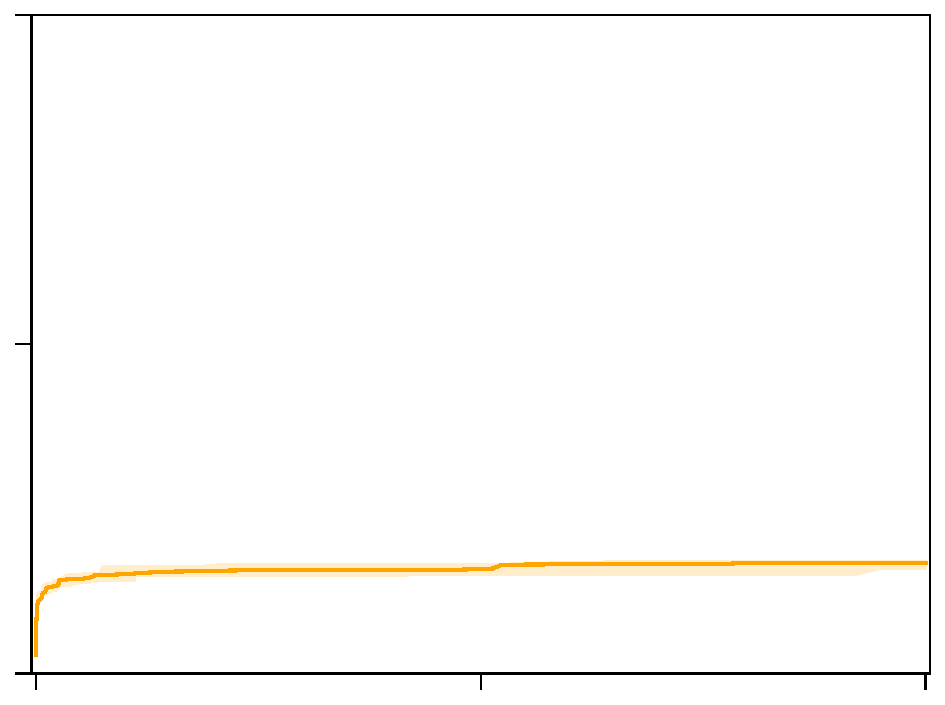
\includegraphics[width=3.1cm]{figures/org_teegris.pdf}
        };
        \node at (beanpod.north) [yshift=0.05cm,xshift=0cm] {\teegris};

        \node[anchor=center] (teegris) at (3.6,0) {
            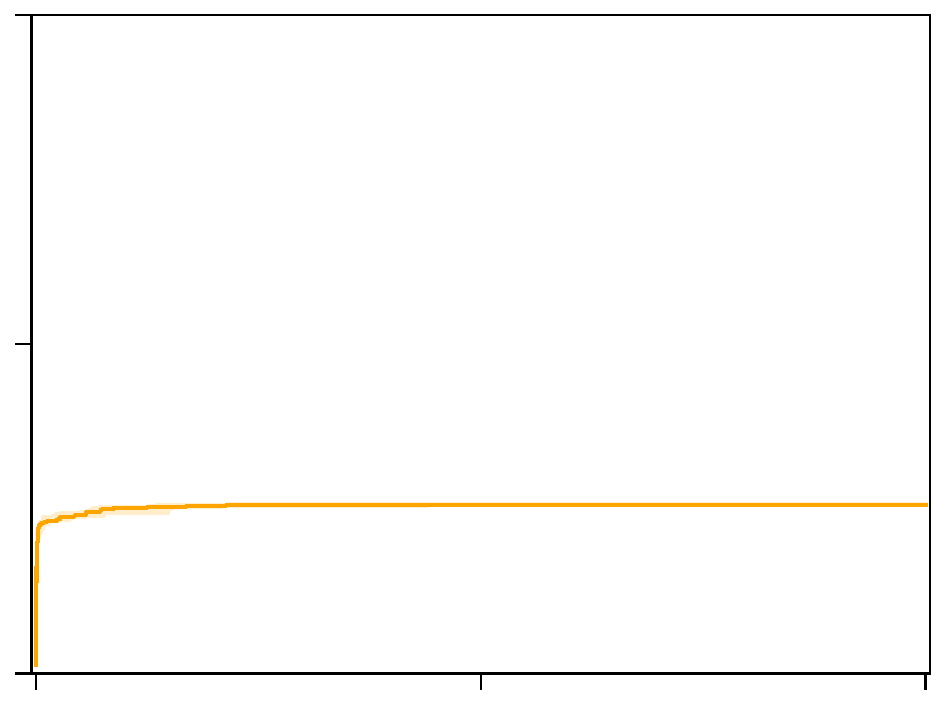
\includegraphics[width=3.1cm]{figures/org_qsee.pdf}
        };
        \node at (teegris.north) [yshift=0.05cm,xshift=0cm] {\qsee};

        \node[anchor=center] (mitee) at (6.9,0) {
            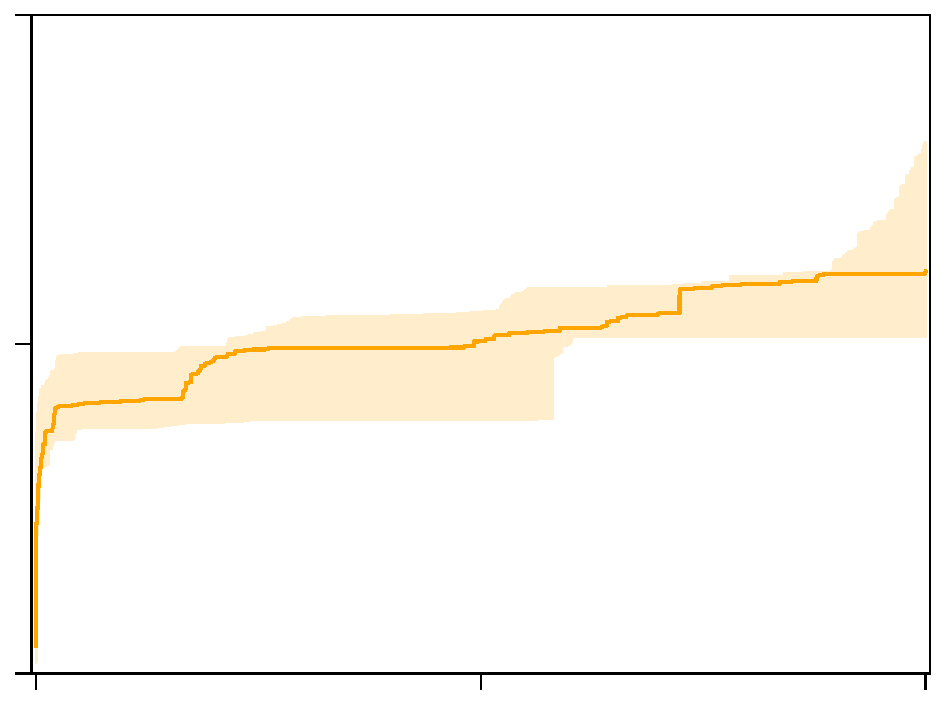
\includegraphics[width=3.1cm]{figures/org_kinibi.pdf}
        };
        \node at (mitee.north) [yshift=0.05cm,xshift=0cm] {\kinibi};

        \node[anchor=center] (beanpod) at (10.2,0) {
            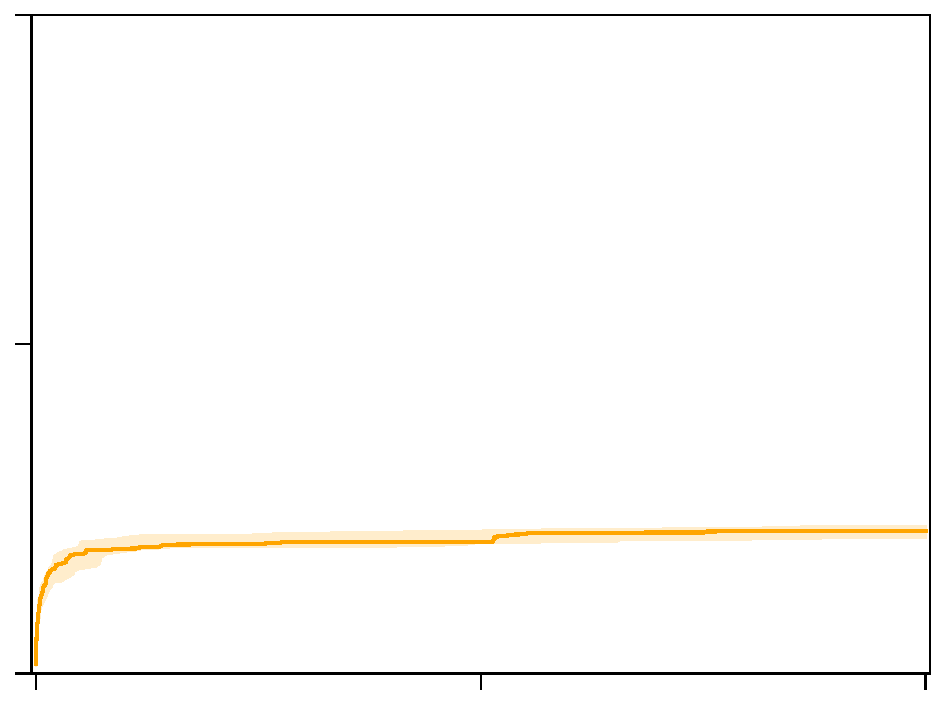
\includegraphics[width=3.1cm]{figures/org_mitee.pdf}
        };
        \node at (beanpod.north) [yshift=0.05cm,xshift=0cm] {\mitee};

        \node[anchor=center] (tsix) at (13.5,0) {
            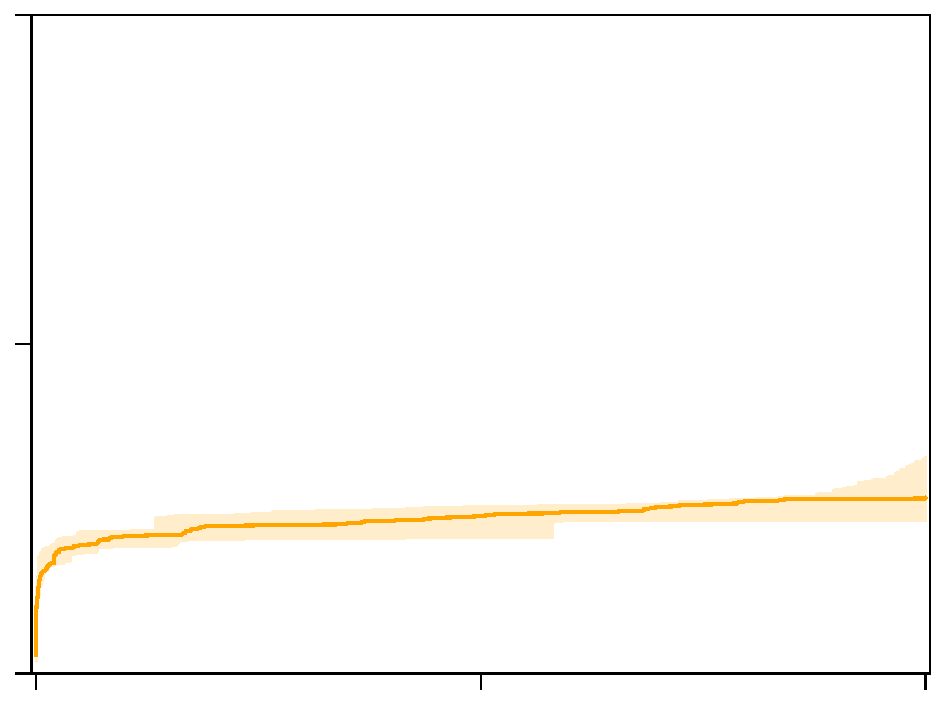
\includegraphics[width=3.1cm]{figures/org_beanpod.pdf}
        };
        \node at (tsix.north) [yshift=0.05cm,xshift=0cm] {\beanpod};

        \node[] at (6.75,-1.5) [] {\footnotesize{Time: 0 to 24 hours}};

    \end{tikzpicture}
    \caption{
        Basic block coverage observed in \stageone. The x-axis denotes the time, and the y-axis is the percentage of covered basic blocks reachable from \texttt{TA\_InvokeCommandEntryPoint}. 
    }
    \label{fig:exploration}
\end{figure*}


\begin{figure*}
    \definecolor{matplotliborange}{rgb}{1.0, 0.647, 0.0}
    \definecolor{matplotlibgreen}{rgb}{0.0, 0.5, 0.0}
    \definecolor{matplotlibblue}{rgb}{0.0, 0.0, 1.0}
    \begin{tikzpicture}

        %\node[] at (-1.5,1.1) [] {\footnotesize{100}};
        %\node[] at (-1.45,0) [] {\footnotesize{50}};
        %\node[] at (-1.4,-1.1) [] {\footnotesize{0}};

        \begin{scope}[shift={(0,0)}]
        \node[anchor=center] (0801) at (0,0) {
            
\includegraphics[width=2.7cm]{figures/df_beanpod_0801_fuzz.pdf}
        };
        \node at (0801.north) [yshift=0.05cm,xshift=0cm] {\beanpod 0801};

        \node[anchor=center] (655a) at (2.8,0) {
            
\includegraphics[width=2.7cm]{figures/df_beanpod_655a_fuzz.pdf}
        };
        \node at (655a.north) [yshift=0.05cm,xshift=0cm] {\beanpod 655a};

        \node[anchor=center] (8aaa) at (5.6,0) {
            
\includegraphics[width=2.7cm]{figures/df_beanpod_8aaa_fuzz.pdf}
        };
        \node at (8aaa.north) [yshift=0.05cm,xshift=0cm] {\beanpod 8aaa};

        \node[anchor=center] (df1e) at (8.4,0) {
            
\includegraphics[width=2.7cm]{figures/df_beanpod_df1e_fuzz.pdf}
        };
        \node at (df1e.north) [yshift=0.05cm,xshift=0cm] {\beanpod df1e};

        \node[anchor=center] (377e) at (11.2,0) {
            
\includegraphics[width=2.7cm]{figures/df_mitee_377e_fuzz.pdf}
        };
        \node at (377e.north) [yshift=0.05cm,xshift=0cm] {\mitee 377e};

        \node[anchor=center] (3d08) at (14,0) {
            
\includegraphics[width=2.7cm]{figures/df_mitee_3d08_fuzz.pdf}
        };
        \node at (3d08.north) [yshift=0.05cm,xshift=0cm] {\mitee 3d08};
        \end{scope}

        \begin{scope}[shift={(0,-2.5)}]
        \node[anchor=center] (655amitee) at (0,0) {
            
\includegraphics[width=2.7cm]{figures/df_mitee_655a_fuzz.pdf}
        };
        \node at (655amitee.north) [yshift=0.05cm,xshift=0cm] {\mitee 655a};

        \node[anchor=center] (86f6) at (2.8,0) {
            
\includegraphics[width=2.7cm]{figures/df_mitee_86f6_fuzz.pdf}
        };
        \node at (86f6.north) [yshift=0.05cm,xshift=0cm] {\mitee 86f6};

        \node[anchor=center] (88ce) at (5.6,0) {
            
\includegraphics[width=2.7cm]{figures/df_mitee_88ce_fuzz.pdf}
        };
        \node at (88ce.north) [yshift=0.05cm,xshift=0cm] {\mitee 88ce};

        \node[anchor=center] (8aaa) at (8.4,0) {
            
\includegraphics[width=2.7cm]{figures/df_mitee_8aaa_fuzz.pdf}
        };
        \node at (8aaa.north) [yshift=0.05cm,xshift=0cm] {\mitee 8aaa};

        \node[anchor=center] (a374) at (11.2,0) {
            
\includegraphics[width=2.7cm]{figures/df_mitee_a374_fuzz.pdf}
        };
        \node at (a374.north) [yshift=0.05cm,xshift=0cm] {\mitee a374};

        \node[anchor=center] (3d08qsee) at (14,0) {
            
\includegraphics[width=2.7cm]{figures/df_qsee_3d08_fuzz.pdf}
        };
        \node at (3d08qsee.north) [yshift=0.05cm,xshift=0cm] {\qsee 3d08};
        \end{scope}
        
        \begin{scope}[shift={(0,-5)}]
        \node[anchor=center] (a985) at (0,0) {
            
\includegraphics[width=2.7cm]{figures/df_qsee_a985_fuzz.pdf}
        };
        \node at (a985.north) [yshift=0.05cm,xshift=0cm] {\qsee a985};

        \node[anchor=center] (4844) at (2.8,0) {
            
\includegraphics[width=2.7cm]{figures/df_teegris_000048444350_fuzz.pdf}
        };
        \node at (4844.north) [yshift=0.05cm,xshift=0cm] {\teegris 4844};

        \node[anchor=center] (4662) at (5.6,0) {
            
\includegraphics[width=2.7cm]{figures/df_teegris_4662436b6d52_fuzz.pdf}
        };
        \node at (4662.north) [yshift=0.05cm,xshift=0cm] {\teegris 4662};

        \node[anchor=center] (5345) at (8.4,0) {
            
\includegraphics[width=2.7cm]{figures/df_teegris_semese_fuzz.pdf}
        };
        \node at (5345.north) [yshift=0.05cm,xshift=0cm] {\teegris 5345};

        \node[anchor=center] (df1ekinibi) at (11.2,0) {
            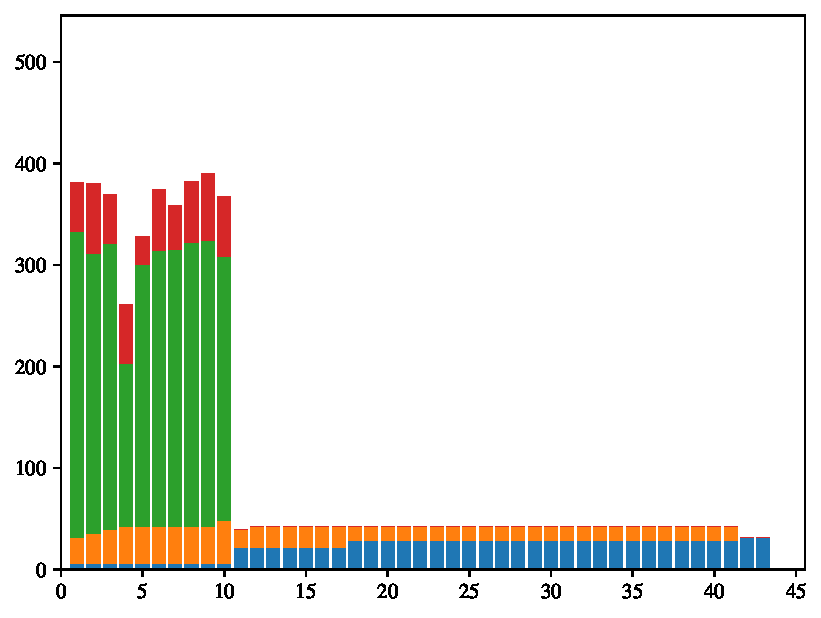
\includegraphics[width=2.7cm]{figures/df_kinibi_df1e_fuzz.pdf}
        };
        \node at (df1ekinibi.north) [yshift=0.05cm,xshift=0cm] {\kinibi df1e};

        \node[anchor=center] (0801kinibi) at (14,0) {
            
\includegraphics[width=2.7cm]{figures/df_kinibi_0801_fuzz.pdf}
        };
        \node at (0801kinibi.north) [yshift=0.05cm,xshift=0cm] {\kinibi df1e};
        \end{scope}
        \node[] at (6.75,-6.3) [] {Snapshots};
        \node[rotate=90, anchor=west] at (-3,-3) [xshift=-1cm, yshift=-1cm] {\# Basic Blocks};

    \end{tikzpicture}
    \caption{
        The basic blocks discovered during \stagetwo. Each graph shows a given fuzzed TA. Each bar corresponds to the basic blocks discovered during \stagetwo for a given snapshot. The y-axis denotes the number of covered basic blocks.  
    \protect\tikz{\fill[matplotlibblue] (0,0) rectangle (0.5cm,0.25cm);} are the basic blocks executed until the second fetch. 
    \protect\tikz{\fill[matplotliborange] (0,0) rectangle (0.5cm,0.25cm);} are basic blocks also covered by the seed that originally triggered the double fetch. 
    \protect\tikz{\fill[matplotlibgreen] (0,0) rectangle (0.5cm,0.25cm);} are basic blocks also covered during \stageone. 
    \protect\tikz{\fill[red] (0,0) rectangle (0.5cm,0.25cm);} are basic blocks \emph{only} covered during \stagetwo. 
    }
    \label{fig:df}
\end{figure*}

\paragraph{Results}

\autoref{tab:dataset} shows the results of the campaign. In total, \sysname detected 
\numTAsdf{} TAs (75\% of the fuzzed TAs) with overlapped fetches. 
After deduplication and merging the \numdfs{} overlapped fetches, \numdfsmerge snapshots 
are passed to \stagetwo. \autoref{fig:exploration} shows the coverage graph from \stageone. 
We estimate the maximally reachable number of basic blocks by building a CFG from each TA's
\texttt{TA\_InvokeCommandEntryPoint} function and counting the unique entrypoint-reachable basic blocks. 
Our harnessing method is able to achieve between 15 - 30\% coverage (except for \kinibi). 
We discuss how this coverage may be further improved in \autoref{sec:discussion}.

In \stagetwo, we fuzz the \numdfsmerge snapshots each for 15 minutes for a total of 4'330 hours. 
\autoref{fig:df} shows the basic blocks covered during \stagetwo for each snapshot. 
We distinguish between four types of covered basic blocks. Especially interesting are the harnesses which covered basic blocks in \stagetwo, which 
were not covered during \stageone, i.e., \sysname discovered code only reachable due to double 
fetches. \stagetwo resulted in \numcrashes crashes. With \stagethree, we narrow these crashes down to \numcrashesdistill crashes only triggerable with shared memory. 
All distilled crashes result from a TOCTTOU vulnerability. \sysname detected TOCTTOU vulnerabilities 
in \numvulnTAs TAs, 15\% of the harnessed TAs.
We manually triage these distilled 
crashes and discover the \numvulns{} vulnerabilities in \autoref{tab:vulns}. 
We further analyzed the remaining 268 non-distilled crashes and found that all of them can be triggered without 
shared memory, arising from conventional bugs in handling input from an untrusted source, confirming that \stagethree 
correctly filters non-TOCTTOU bugs. Note that \sysname may discover non-TOCTTOU vulnerabilities both during 
\stageone and \stagetwo. We have triaged and reported \emph{all} discovered crashes to the affected vendors.

\begin{table*}[t]
    \small
    \centering
    %\begin{adjustbox}{max width=\columnwidth}
    \begin{tabular}{llllc}
        TEE&
        TA UUID &
        TA Name & 
        DF Vulnerability &
        \makecell{Reproduced\\on Device} \\
        \midrule
        \mitee      & 377ee4e8-af0e-474f-a9d636a9268fe85c   & SoterApp & stack overflow    & \checkmark \\
        \teegris    & 00000000-0000-0000-0000-4662436b6d52  & FbSkmR & oob read          & \checkmark \\
        \mitee,\qsee& 3d08821c-33a6-11e6-a1fa089e01c83aa2   & VSIMApp & oob write         & \checkmark* \\
        \mitee,\qsee& 3d08821c-33a6-11e6-a1fa089e01c83aa2   & VSIMApp & double free       & \checkmark* \\
        \mitee      & 88ce8e6b-8646-4092-bb78faf5b55ff4df   & Mlipay & oob read          & \checkmark \\
        \kinibi,\beanpod   & 08010203000000000000000000000000       & ifaa-key & oob read          & \xmark \dag \\
        \bottomrule
    \end{tabular}
    %\end{adjustbox}
    \caption{
    The vulnerabilities in commercial TAs found with \sysname.
    (*) Only on \mitee, because we did not have a \qsee testing device supporting this TA.
    (\dag) None of our testing devices supports the TA. 
    }
    \label{tab:vulns}
\end{table*}

% stats of campaign

% coverage graphs

\subsection{Reproducing DF Vulnerabilities on Phones}

\begin{table}[t]
    \small
    \centering
    %\begin{adjustbox}{max width=\columnwidth}
    \begin{tabular}{llc}
        TEE&
        Phone &
        Zero-Copy Shm\\
        \midrule
        \teegris    & Samsung A56 5G   & \checkmark \\
        \teegris    & Samsung A16   & \checkmark \\
        \teegris    & Samsung S22   & \checkmark \\
        \teegris    & Samsung S10   & \checkmark \\
        \qsee       & OnePlus 12R   & \checkmark \\
        \qsee       & OnePlus Nord 5  & \checkmark \\
        \kinibi     & Transsion Pova Pro 5   & \checkmark \\
        \kinibi     & Transsion Infinix Note 12   & \checkmark \\
        \mitee      & Xiaomi 15T   & \checkmark \\
        \mitee      & Xiaomi Redmi Note 13 5G   & \checkmark \\
        \beanpod    & Xiaomi Redmi Note 11s 5G  & \xmark \\
        \beanpod    & Xiaomi Redmi 9A  & \xmark \\
        \bottomrule
    \end{tabular}
    %\end{adjustbox}
    \caption{
        The devices we used to reproduce double fetches. All devices were updated to the newest firmware version. 
    }
    \label{tab:phones}
\end{table}

\begin{listing}[ht]
    \definecolor{pgreen}{rgb}{0,0.5,0}
\definecolor{pblue}{rgb}{0.13,0.13,1}
\definecolor{pred}{rgb}{0.9,0,0}
\definecolor{pgrey}{rgb}{0.46,0.45,0.48}
\definecolor{light-gray}{gray}{0.975} \definecolor{darkgreen}{rgb}{0,0.5,0}
\definecolor{vscodepurple}{RGB}{128, 0, 128}
\definecolor{codepurple}{rgb}{0.58,0,0.82}

\lstset{escapechar=@,
                backgroundcolor = \color{light-gray},
                %linebackgroundcolor={%
                %\ifnum\value{lstnumber}>0
                %    \ifnum\value{lstnumber}<30
                %        \color{light-gray}
                %    \fi
                %\fi
                %}
                tabsize=2,
                basicstyle=\fontencoding{T1}\selectfont\footnotesize,
                %basicstyle=\fontfamily{lmvtt}\selectfont\footnotesize,
                commentstyle=\color{darkgreen!80},
                keywordstyle=\color{pblue},
                stringstyle=\color{pred},
                %stringstyle=\color{vscodepurple},
                frame = single,
                showstringspaces=false,
                language=c,
                xleftmargin=5pt, 
                xrightmargin=5pt, 
                %framexleftmargin=-5pt,
                numbers=left,                  % Line numbers
                numberstyle=\tiny\color{black}, % Line number style
                numbersep=4pt, %moredelim=[is][\textbf]{@}{@}
                %escapeinside={(*@}{@*)}
}
\center

\begin{lstlisting}[columns=fullflexible]
void* mod_thread(void* shm){
  while(1){
    mod1(shm);
    mod2(shm);
  }
}
typedef struct imp_shm{
  uint64_t _ignore[3];
  void* shm;
}
void trigger_df(TEEC_Context *context, 
    TEEC_Session *session, cmd){
  TEEC_SharedMemory in_mem;
  in_mem.size = buf_size;
  in_mem.flags = TEEC_MEM_INPUT; 
  res = TEEC_AllocateSharedMemory(context, &in_mem);
  if (res != TEEC_SUCCESS) exit(-1);
  imp_shm* imp = in_mem->imp;
  void* shm = imp->shm;
    
  pthread_t tid;
  pthread_create(&tid, NULL, mod_thread, shm);
  
  setup_params(&op, &in_mem);
  TEEC_InvokeCommand_impl(session, cmd, &op, &err_origin);
}

int main(){
  TEEC_Context context; TEEC_Session session;
  open_session(&context, &session);
  trigger_df(&context, &session);
}
\end{lstlisting}
                                                                                  
    \captionof{lstlisting}{
        The relevant components of our POC to trigger double fetch vulnerabilities.
    }
    \label{lst:poc}
\end{listing}

Our implementation of \sysname assumes that \texttt{memref} buffers are zero-copy shared memory. 
However, as discussed in \autoref{sec:background}, the TEE implementation may 
make a local copy of the buffer. To demonstrate that the findings by \sysname 
are actual security vulnerabilities, we need to trigger the TOCTTOU  
vulnerabilities on COTS devices. See \autoref{tab:phones} for the devices 
we used in this evaluation. All devices are rooted and updated to the newest 
firmware version.  
Our Proof-Of-Concept (POC) NWCA runs on the testing device and attempts to trigger the TOCTTOU  
vulnerabilities. It implements three functionalities: 
obtaining a pointer to shared memory, invoking the vulnerable TA functionality, 
and racing the shared memory access. 

To communicate with the TA, our POC uses the GlobalPlatform client library shipped on the device. 
The GlobalPlatform client library is developed by the TEE vendor to correctly interface with 
the TEE-specific kernel driver. With this library, GlobalPlatform-compliant 
NWCAs can use the GlobalPlatform APIs to communicate with the TAs. By leveraging the client library, we can reuse most
parts of the POC for different TEEs. To obtain a pointer to shared memory, our POC 
leverages the \texttt{TEEC\_AllocateSharedMemory} API to allocate a memory buffer 
shared with the TA. 

We find that both the GlobalPlatform client library for \mitee 
and \teegris do not return a pointer to the actual shared memory in this API. 
Instead, a pointer to an intermediate buffer is returned, whose content is copied 
to the actual shared memory (shared with the TA) by the client library when invoking the TA 
functionality. This way of hiding the true shared memory buffer is not secure against a malicious 
NWCA and removes the option of zero-copy shared memory for benign use cases. 
%To obtain the pointer to shared memory, we reverse engineer the 
%GlobalPlatform client libraries and in the POC retrieve the true shared memory pointer ourselves. 
\autoref{lst:poc}, Lines 13 to 19, show how our POC retrieves the pointer to shared memory.

%It first retrieves the TEE-specific \texttt{imp} pointer from the shared memory structure (\texttt{in\_mem}), 
%and then uses the reverse-engineered struct (\texttt{imp\_shm}) to retrieve the actual 
%shared memory pointer. Note that the Listing shows the structure for \teegris, it is different 
%for the other TEEs.

%\mb{The details here are a bit verbose and distract from the actual experiment that answers the research question. We can shorten this by just saying that references to zero-copy shared memory were accessible in the NWCA context of the corresponding TEEs. The details about reversing this can go in the appendix.}

%\begin{figure}[t]
%  \centering
%  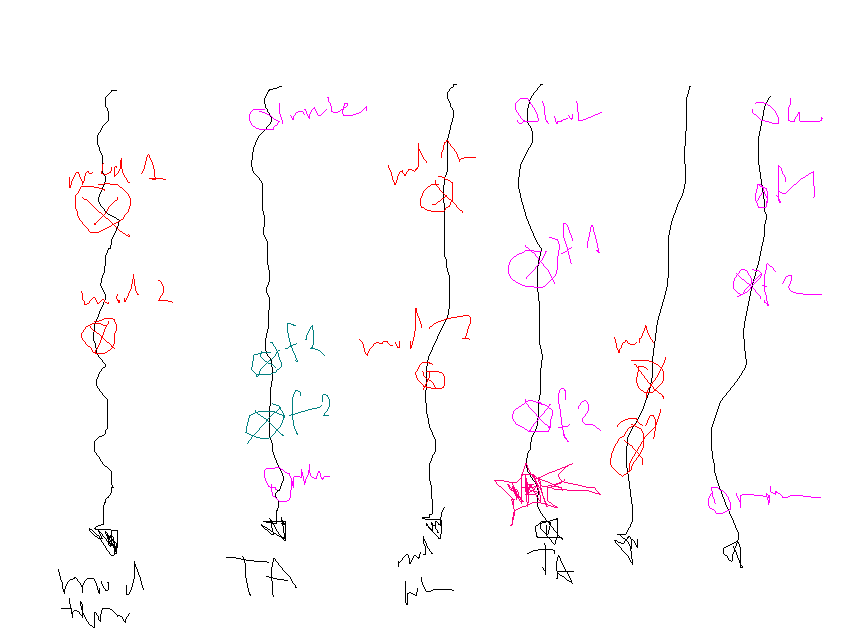
\includegraphics[width=0.46\textwidth]{figures/race_vis.png}
%  \caption{
%    \mao{fix figure}
%    \mao{
%    actually only four scenarios, but slightly different}
%    The scenarios that our POC's racing thread triggers. 
%    In scenario \mao{TODO} the TA's double fetch vulnerability is 
%    triggered. 
%  }
%  \label{fig:racevis}
%\end{figure}

After obtaining the shared memory pointer, 
our POC spawns a separate thread that asynchronously modifies the shared 
memory while the TA is operating on it. This way, we can race the 
double fetch accesses and eventually trigger the TOCTTOU vulnerability. 
Lines 1 to 6 in \autoref{lst:poc} show the racing thread. \texttt{Mod1} sets up the shared memory such that the TA's 
check passes, while \texttt{mod2} modifies shared memory to cause a crash during use.
If \texttt{mod2} happens between 
the fetches of the TA, the TA reads two different values, thus triggering 
the TOCTTOU vulnerability.

Finally, the POC invokes the TA's vulnerable functionality. We need to correctly 
set up the expected arguments. To populate the arguments, we leverage the fuzzer-generated 
seed that triggered the double fetch (Lines 24 to 25 in \autoref{lst:poc}).
We write our POC such that triggering the double fetch vulnerability will 
cause the TA to crash. To observe if we caused the TA to crash, we check the 
return code of the \texttt{TEEC\_InvokeCommand} function. \footnote{a return value of \texttt{0xFFFF3024} (\texttt{TEE\_ERROR\_TARGET\_DEAD}) indicates the TA has crashed.~\cite{gpintapi}}
We run the POC in a loop until we observe a crash. 
We reproduce \numvulnsrepro{} out of \numvulns{} discovered 
double fetch vulnerabilities on-device, see \autoref{tab:vulns}.

\paragraph{Case Study: Stack-based Overflow \mitee}

\begin{listing}[h]
    \input{listings/soterbug.tex}
    \captionof{lstlisting}{
        The simplified code of the double fetch stack overflow vulnerability in the 
        SoterApp TA. 
        The \texttt{shm} argument of the function points to the shared \texttt{memref} buffer. 
    }
    \label{lst:soterbug}
\end{listing}

The affected TA has a TOCTTOU vulnerability 
leading to a stack-based buffer overflow. \autoref{lst:soterbug} shows the vulnerable code. 
The TA first obtains the length of the null-terminated string in shared memory during the first 
fetch. As part of the second fetch, the TA copies a string from shared memory into a stack buffer. 
To trigger the stack-based buffer overflow, our POC's \texttt{mod\_thread} sets up the shared 
memory with a string larger than 0x80. It then repeatedly sets the 
first byte in the shared memory to 0 and back to the original string value. If the fetches 
line up, \texttt{strlen} is calculated on a zero-length string, but \texttt{strcpy} will 
copy a string larger than 0x80, triggering the stack-based buffer overflow.

\paragraph{Case Study, OOB read \teegris}

\begin{listing}[h]
    \definecolor{pgreen}{rgb}{0,0.5,0}
\definecolor{pblue}{rgb}{0.13,0.13,1}
\definecolor{pred}{rgb}{0.9,0,0}
\definecolor{pgrey}{rgb}{0.46,0.45,0.48}
\definecolor{light-gray}{gray}{0.975}
\definecolor{darkgreen}{rgb}{0,0.5,0}
\definecolor{vscodepurple}{RGB}{128, 0, 128}
\definecolor{codepurple}{rgb}{0.58,0,0.82}

\lstset{escapechar=@,
                backgroundcolor = \color{light-gray},
                linebackgroundcolor={%
                \ifnum\value{lstnumber}>0
                    \ifnum\value{lstnumber}<30
                        \color{light-gray}
                    \fi
                \fi
                %\ifnum\value{lstnumber}>10
                %    \ifnum\value{lstnumber}<12
                %        \color{teal!40}
                %    \fi
                %\fi
                \ifnum\value{lstnumber}>3
                    \ifnum\value{lstnumber}<5
                        \color{blue!20}
                    \fi
                \fi 
                \ifnum\value{lstnumber}>4
                    \ifnum\value{lstnumber}<6
                        \color{red!20}
                    \fi
                \fi
                },
                tabsize=2,
                basicstyle=\fontencoding{T1}\selectfont\footnotesize,
                %basicstyle=\fontfamily{lmvtt}\selectfont\footnotesize,
                commentstyle=\color{darkgreen!80},
                keywordstyle=\color{pblue},
                stringstyle=\color{pred},
                %stringstyle=\color{vscodepurple},
                frame = single,
                showstringspaces=false,
                language=c,
                xleftmargin=5pt, 
                xrightmargin=5pt, 
                %framexleftmargin=-5pt,
                numbers=left,                  % Line numbers
                numberstyle=\tiny\color{black}, % Line number style
                numbersep=4pt, %moredelim=[is][\textbf]{@}{@}
                %escapeinside={(*@}{@*)}
}
\center

\begin{lstlisting}[columns=fullflexible]
TEE_Result TA_InvokeCommandEntryPoint(.., params){
  void* buf0 = params[0].memref.buffer;
  size_t buf0_size = params[0].memref.size;
  if(*(size_t*)buf0 > buf0_size) return -1;
  size_t ser_size = *(size_t*)buf0;
  void* local = TEE_Malloc(ser_size);
  memcpy(local, buf0, ser_size);
  ...
}
\end{lstlisting}

    \captionof{lstlisting}{
        The simplified code of the double fetch out-of-bound read vulnerability in the 
        FbSkmR TA. 
    }
    \label{lst:teegrisbug}
\end{listing}

The affected \teegris TA has a TOCTTOU vulnerability leading to an out-of-bounds read on the 
input shared memory buffer. The TA expects the input buffer to contain length-value 
serialized data. It first checks if the 
serialized length is not larger than the size of the shared memory buffer at Line 4 (\autoref{lst:teegrisbug}).
The TA then fetches the length again at Line 5 and copies from the shared memory buffer to 
a local buffer. The \texttt{mod\_thread} for this TA's POC repeatedly sets the 
first \texttt{size\_t} value in the shared memory to zero or a very large value, 
which will crash in the \texttt{memcpy} function when reading out of bounds of the buffer.

\paragraph{Double Fetches in other TEEs}

For the TEEs for which we did not reproduce a crash on-device (\kinibi, \beanpod, and 
\qsee), either due to \sysname not finding a crash or the vulnerable TA not 
being supported on our testing devices, we still want to test if the TEE supports 
zero-copy shared memory. To this end, we manually analyze the overlapped fetches found 
in TAs from these TEEs to find fetches that, if triggered, lead to an observable 
outcome. We find that both \kinibi and \qsee support zero-copy shared memory, see Appendix~\ref{sec:qseekinibidf} 
for the details of the double fetches we used. However, \beanpod does not support 
shared memory. We leverage the exploit from~\cite{globalconfusion} to 
achieve code execution in a \beanpod TA. Our shellcode repeatedly reads from the 
\texttt{memref} buffer and logs the value. Although we are modifying the value concurrently
from our NWCA, we are unable to observe changes in the \texttt{memref} buffer accessed by the TA.
The results of this evaluation on the availability of zero-copy shared memory in major TEEs 
can be found in \autoref{tab:phones}.

% beanpod -> tested and no
% kinibi -> tested and yes
% qsee -> TODO
% t6 -> maybe ?

\subsection{Memory-Safe TAs}

\begin{table*}[ht]
    \footnotesize
    \centering
    %\begin{adjustbox}{max width=\columnwidth}
    \begin{tabular}{llr}
        \toprule
        TA&
        SHM Operation&
        \# Detected Double Fetches\\ 
        \toprule
        message\_passing\_interface-rs & \texttt{serde\_json::from\_slice} & 490 \\
        eth\_wallet & \texttt{bincode::deserialize} & 0 \\
        mnist-rs & \texttt{bytemuck::cast\_slice} & 0 \\
        udp/tcp\_client-rs* & \texttt{core::str::from\_utf8} & 351 \\
        Bitcoin-Wallet-for-Trusted-OS-OPTEE & \makecell{custom deserialize and  signing} & 1 \\
        \bottomrule
    \end{tabular}
    %\end{adjustbox}
    \caption{
        The Rust TAs that operate on shared memory. The "SHM Operation" column denotes either the API 
        called on the shared memory slice or the operations on said slice.
        (*) We only fuzz the tcp\_client TA since the udp TA has an identical operation on shared memory.
    }
    \label{tab:rust}
\end{table*}

All the COTS TAs analyzed so far are written in C/C++. In the future, stakeholders 
(vendors, developers) may move to address memory corruption vulnerabilities, the most widely 
exploited category of vulnerabilities, in TAs, by reimplementing them in a memory-safe language.
However, irrespective of the language in which the TA is written, the underlying shared memory 
API design still exposes the TA to a pointer shared with the untrusted normal world. This  
pointer may be abstracted by the language, and thus the fact that it is shared is hidden from the developer. 
To understand how shared memory double fetches affect TAs written in memory-safe languages, we analyze 
TAs written in Rust.
While we did not observe any Rust TAs deployed on 
COTS devices, we believe that the TEE space will start adopting 
Rust, just as is the case for other Android components such as 
parts of the Linux kernel~\cite{rustbinder} or of the user space~\cite{rustandroid}.

%\ed{To me, the programming language is orthogonal to the physical implementation. 
%Rust should be just as vulnerable as C, under the same security assumptions, i.e. assuming
%that reading from a shmem buffer can lead to double fetch issues.
%Wouldn't this issue also occur in any programming language, even in, say e.g. java, if the buffer is treated as zero-copy shared memory?
%To my understanding it is a clear API design issue that must be addressed (as you correctly do below). 
%The programming language is not at fault, as it abstracts this behavior altogether.
%Introducing the same API for Rust would similarly get rid of this attack vector, if I understand correctly.
%}

%\mb{more context, we don't say yet explicitly that in the context of our research it comes as a natural question to investigate the susceptibility of Rust TAs for double-fetch bugs.}

Apache Teaclave~\cite{rustee,teaclave} is the official SDK for writing TAs in Rust for \optee.
\optee is the reference TrustZone TEE implementation and most 
TEEs deployed on COTS devices are derived from \optee. 
It follows that Rust TAs for commercial TEEs will be derivatives  
of \optee's Rust TA SDK. We inspect the Teaclave SDK and find 
that TAs obtain a mutable \texttt{[u8]} slice when accessing 
the \texttt{memref} buffer. This slice is obtained using the 
\texttt{std::slice from\_raw\_parts\_mut} API, with the 
\texttt{memref}'s buffer pointer and size. The Rust documentation 
states the following in the safety section of \texttt{from\_raw\_parts\_mut}~\cite{rustfromraw}: 

\begin{tcolorbox}                                                                                                                   
The memory referenced by the returned slice must not be accessed through any other pointer (not derived from the return value) for the duration of lifetime \texttt{'a}. Both read and write accesses are forbidden.
\end{tcolorbox}

This requirement is violated when the mutable slice is derived from a 
pointer to shared memory, since the NWCA has a pointer to the 
slice's underlying physical memory and may read/write to it. 
Thus, for TAs written in Rust, which operate directly on the shared 
memory slice, the Rust compiler can not give any safety guarantees.

We inspect \numRustTAs TAs written in Rust (part of the 
Teaclave reference examples or independent Github projects~\cite{teaclave,bitcoinrust}) and 
check if the TAs operate on shared memory directly or make a copy. 
We find that \numRustTAsnoShm TAs use APIs such as \texttt{to\_vec} to make a local copy of the buffer. 
\numRustTAsShm TAs operate directly on shared memory in Rust, deserializing data directly from the 
shared memory buffer. 
We fuzz these TAs with \sysname to understand if the Rust code has double fetches. 
\autoref{tab:rust} shows the results. Four of the six TAs have double fetches. 
% validation in utf8 double check

While \sysname did not trigger any crashes during \stagetwo, manually analyzing the 
overlapped fetches, we found that in three out of four TAs, these double fetches lead to TOCTTOU logic bugs.
The double fetches in the udp/tcp\_client TAs happen due to the fact that \texttt{core::str::from\_utf8} 
first traverses the shared memory slice to ensure it contains valid UTF-8. Afterwards, the API just 
returns a pointer to the underlying slice. If the TA afterwards accesses the string, 
its contents may have been changed to invalid UTF-8. 
The Bitcoin-Wallet-for-Trusted-OS-OPTEE TA deserializes a \texttt{Transaction} object directly from the 
shared memory buffer. Afterwards, the TA refetches the entire shared memory and signs the transaction 
data. In between the two fetches, an attacker can modify the shared memory, and thus the TA will 
sign arbitrary attacker-controlled data instead of a correctly deserialized transaction.
%For the \texttt{serde\_json} deserialization in the message\_passing TA, the double fetch is 
%related to an error condition, which rechecks memory and can only be used to turn an invalid 
%json into a valid one.
 
Our results demonstrate that even TAs written in memory-safe languages, such as Rust, are affected by double fetches. 
%We emphasize that the TAs analyzed in this section are not deployed on COTS devices and serve as reference examples. 
%Nevertheless, the fact that even these minimal TAs are affected—and exhibit 
%logic bugs—underscores the severity of double-fetch vulnerabilities in memory-safe TAs.


%pub fn buffer(&mut self) -> &mut [u8] {
 %       unsafe { slice::from_raw_parts_mut((*self.raw).buffer as *mut u8, (*self.raw).size) }
 %   }
%
%


%%%%%%%%%%%%%%%%%%%%%%%%%%%%%%%%%%%%%%%%%%%%%%%%%%%%%%%%%%%%%%%%%%%%%%%%%%%%%%%%
\section{Mitigation}\label{sec:mitigation}
%%%%%%%%%%%%%%%%%%%%%%%%%%%%%%%%%%%%%%%%%%%%%%%%%%%%%%%%%%%%%%%%%%%%%%%%%%%%%%%%

As demonstrated in \autoref{sec:evaluation}, vulnerabilities due to shared memory 
double fetches are an insidious problem plaguing TAs, both for TAs currently 
deployed on COTS phones and future TAs written in memory-safe languages.
Analysis of the discovered 
vulnerabilities revealed that the affected TAs do not rely on zero-copy shared 
memory for their functionality. Instead, it appears the TA developer did not 
consider the \texttt{memref} buffer to be shared.

This is not the developer's fault. Instead, it is an oversight of the GlobalPlatform specification and 
the TEE implementations, which obscure the fact that \texttt{memref} buffers may 
be shared. First, TEE implementations may or may not implement zero-copy shared 
memory. A TA developed for a TEE without zero-copy shared memory may later be 
deployed on a TEE with shared memory, or the TEE itself may switch to zero-copy 
shared memory in a later version. Furthermore, while there is a warning in the 
GlobalPlatform specification~\cite{gpintapi}, the proposed solution is ineffective. The document 
suggests using \texttt{TEE\_CheckMemoryAccessRights} to check 
if a memory region is shared with a NWCA. By \emph{not} setting the \texttt{TEE\_MEMORY\_ACCESS\_ANY\_OWNER} 
flag, the API returns -1 if the memory is shared. It  
is unclear to us whether TEEs support this flag, since we have not 
found a single TA in our dataset calling this API to check for shared memory. 

\begin{figure}[]
  \centering
  \input{figures/mitigation.tex}
  \caption{
    An overview of our mitigation. A TA may register \texttt{memref} buffers of 
    one or more specific commands as zero-copy shared memory using \texttt{RegisterShm}.
    When the NWCA invokes the TA, the TEE runtime checks if the input buffers were registered, 
    creating a local copy if not.
    }
  \label{fig:mitigation}
\end{figure}

Instead of leaving shared memory handling to developers and obscure APIs, we propose 
to mitigate this design weakness with an extension to the GlobalPlatform specification. This extension 
makes zero-copy shared memory explicit, removing ambiguity on shared memory and 
ensuring that double fetches on \texttt{memref} buffers are not a security issue by 
default. If a TA developer wishes to make use of zero-copy shared memory, the developer 
needs to explicitly register a \texttt{commandID},
\texttt{memref} buffer combination as zero-copy shared memory with the TEE runtime. 
For \texttt{memref} buffers not registered, the TEE runtime will create a local 
copy of the buffer and pass the local buffer to the TA. This extension changes 
the shared memory model to a fail-closed design, meaning that TAs that do not 
consider shared memory will \textbf{not} have double fetch vulnerabilities. 
Essentially, it makes the two scenarios outlined in~\autoref{fig:shmex} explicit 
to the developer. Our mitigation fixes all vulnerabilities discovered by \sysname, 
without changes to the existing TAs.

To demonstrate the feasibility of our mitigation, we implement it for \optee, the 
reference GlobalPlatform-compliant TEE implementation. We add a new API \texttt{TEE\_RegisterShm}, 
which allows a TA to register an entry in the \texttt{params} array for a given 
\texttt{commandID} as shared. In its \texttt{TA\_CreateEntryPoint} function, the 
TA registers the \texttt{memref} that needs to be zero-copy shared memory. 
\autoref{lst:mitigta} shows how a TA leverages this new API to request a
zero-copy shared memory buffer. When the TA's \texttt{TA\_InvokeCommandEntryPoint} function is called, the TEE user 
space runtime checks for each \texttt{memref} parameter, if for the given 
\texttt{commandID}, the \texttt{memref} was registered as zero-copy shared memory. 
If yes, the runtime passes the pointer to the shared memory to the TA. 
If not, the runtime makes a local copy of the 
buffer and sets the pointer in \texttt{memref} to the local buffer.
\autoref{fig:mitigation} shows how our mitigation works.
Our patch to \optee adds this mitigation in 140 lines 
of code.
We have submitted our mitigation proposal to the GlobalPlatform alliance and are 
in active discussion with them to update the GlobalPlatform TEE internal core 
specification to address shared memory.

\begin{listing}[h]
    \input{listings/mitigta.tex}
    \captionof{lstlisting}{
        The updated \texttt{TA\_CreateEntryPoint} function of the TA from 
        \autoref{lst:exdf}, which explicitly registers the first \texttt{memref}
        buffer when handling command 3 as zero-copy shared memory. All the other 
        \texttt{memref} buffers are not zero-copy, and thus the double fetch bugs 
        in commands 1 and 2 are mitigated.
    }
    \label{lst:mitigta}
\end{listing}

%%%%%%%%%%%%%%%%%%%%%%%%%%%%%%%%%%%%%%%%%%%%%%%%%%%%%%%%%%%%%%%%%%%%%%%%%%%%%%%%
\section{Discussion}\label{sec:discussion}
%%%%%%%%%%%%%%%%%%%%%%%%%%%%%%%%%%%%%%%%%%%%%%%%%%%%%%%%%%%%%%%%%%%%%%%%%%%%%%%%

\paragraph{Beyond Shared Memref Buffers}
In this study, we focus on the normal world reachable attack surface exposed by 
GlobalPlatform-compliant TAs handling shared memory buffers. 
Besides GlobalPlatform-compliant TAs, \kinibi and \qsee support non-compliant TAs, 
whose API may also support zero-copy shared memory. Extending 
\sysname for such TAs is a matter of engineering effort to support loading and 
these TAs in \sysname's emulator component. 

Besides the attack surface of TAs, the TEE 
itself handles shared memory for any other communication with the normal world, 
such as when loading a TA from the normal world file system. We leave auditing 
these shared memory interactions to future work.

\paragraph{\sysname Compared to Reshaping-based Fuzzing Approaches}

Reshaping-based fuzzing approaches~\cite{morphuzz, chen2024enclavefuzz} 
inject fuzzing inputs at memory reads that access 
attacker-controlled memory and are capable of dynamically triggering TOCTTOU vulnerabilities. 
Unlike \sysname, reshaping-based techniques cannot directly target individual double fetch "use" 
instances. They rely on re-executing seed inputs to probabilistically 
re-trigger double fetches. In contrast, \sysname's snapshot-based double fetch fuzzing 
enables specifically targeting double fetches without having to reexecute the target until 
the second fetch occurs. 

To quantify this difference, we measure 
how often double fetches are triggered during exploration. \autoref{tab:reshape} shows the results 
across all harnesses for which we detected overlapped fetches, fuzzed for the same time as during 
\stagetwo for the evaluation in ~\autoref{sec:cotsfuzz}. Across all harnesses, only 
\numexecsdfperc{} of fuzzing iterations actually execute a code path containing a double 
fetch. Since our study targets double fetch vulnerabilities, reshaping-based 
approaches would spend the majority of their effort on executions that cannot trigger the 
vulnerability of interest. 

In its current form, \sysname is unable to detect nested double fetch vulnerabilities, i.e., double fetches 
that are reachable only after triggering another double fetch bug. Reshaping approaches 
can trigger such nested double fetches. Extending \sysname for nested double fetches is possible 
by collecting snapshots during \stagetwo. We deliberately opted to focus on single TOCTTOU 
vulnerabilities to ensure we were able to reproduce our findings on COTS devices. 

\begin{table}[t]
    \footnotesize
    \centering
    %\begin{adjustbox}{max width=\columnwidth}
    \begin{tabular}{lrrr}
        \toprule
        TA&
        \# Execs &
        \# Execs DF &
        Execs DF \%\\
        \toprule
        \fivethreefourfive & \numexecsfivethreefourfive &\numexecsdffivethreefourfive  & \numexecsdfpercfivethreefourfive\\
        \eightaaa & \numexecseightaaa &\numexecsdfeightaaa  & \numexecsdfperceightaaa\\
        \threesevensevene & \numexecsthreesevensevene &\numexecsdfthreesevensevene  &\numexecsdfpercthreesevensevene\\
        \anineeightfive & \numexecsanineeightfive &\numexecsdfanineeightfive  &\numexecsdfpercanineeightfive\\
        \aseventhreefour & \numexecsaseventhreefour &\numexecsdfaseventhreefour  &\numexecsdfpercaseventhreefour\\
        \foursixsixtwo & \numexecsfoursixsixtwo &\numexecsdffoursixsixtwo  &\numexecsdfpercfoursixsixtwo\\
        \eighteigthce & \numexecseighteightce  & \numexecsdfeighteightce &\numexecsdfperceighteightce\\
        \zeroeightzeroone & \numexecszeroeightzeroone &\numexecsdfzeroeightzeroone  &\numexecsdfperczeroeightzeroone\\
        \onefourbzero & \numexecsonefourbzero &\numexecsdfonefourbzero  &\numexecsdfperconefourbzero\\
        \dfonee & \numexecsdfonee &\numexecsdfdfonee  &\numexecsdfpercdfonee\\
        \threedzeroeight & \numexecsthreedzeroeight  & \numexecsdfthreedzeroeight &\numexecsdfpercthreedzeroeight\\
        \foureightfourfour & \numexecsfoureightfourfour &\numexecsdffoureightfourfour  &\numexecsdfpercfoureightfourfour\\
        \sixfivefivea & \numexecssixfivefivea &\numexecsdfsixfivefivea  &\numexecsdfpercsixfivefivea\\
        
        \bottomrule
    \end{tabular}
    %\end{adjustbox}
    \caption{
        The overall executions and executions triggering overlapped fetches resulting from fuzzing the harnesses with overlapped 
        fetches for the same CPU time as during the \stagetwo campaign in \autoref{sec:cotsfuzz}. 
    }
    \label{tab:reshape}
\end{table}


\paragraph{Harnessing TAs for Exploration}
As pointed out by related work~\cite{teezz,syncemu}, TAs may 
expect specific input formats in the input buffers or only expose certain functionality 
in specific states. Our current approach to harnessing does not take this into account; we fuzz 
one invocation of \texttt{TA\_InvokeCommandEntryPoint}, directly inserting fuzzer-mutated bytes 
into the shared memory buffer. As such, the current harnesses are limited in their ability to 
explore TAs, and the number of double fetches detected in~\autoref{sec:evaluation} should 
be viewed as a lower bound. We leave extending \sysname with type/state-aware harnesses to 
future work. 
%However, we show that even with such a simple approach to harnessing, we were still 
%able to detect \numvulns{} vulnerabilities.
%, emphasizing thecriticality of double fetch vulnerabilities in TAs.

\paragraph{Non-Nemory Corruption Double Fetch Bugs}
In its current design, \sysname uses memory safety oracles to detect double fetch vulnerabilities. 
However, double fetches may trigger security-relevant non-memory corruption 
bugs, such as logic bugs. \sysname could automatically detect such vulnerabilities if 
the corresponding bug oracles are implemented in the emulator component. Designing and implementing 
bug oracles for non-memory corruption bugs in TAs is orthogonal to our work. We choose to 
focus on double fetches leading to memory corruptions as this category of vulnerability has 
historically been the most critical one for TA security.

%Second, reshaping-based approaches may expose vulnerabilities involving nested or cascading
%double fetches. While such bugs are theoretically interesting, they are difficult to reproduce
%reliably. \sysname intentionally focuses on single,
%reproducible double-fetch vulnerabilities that can be confirmed on real-world hardware.
%Nevertheless, \sysname can be extended to support nested double fetches by
%recursively snapshotting additional double-fetch sites during \stagetwo.

%Reshaping-based fuzzing appraoches such as EnclaveFuzz~\cite{chen2024enclavefuzz} or 
%MORPHUZZ~\cite{morphuzz} fuzz the target and inject fuzzing data on memory-reads
%accessing of attacker-controlled memory. These approaches can find double 
%fetch vulnerabilities dynamically. However, one, unable to target a specific double 
%fetch, snapshot can target specific fetch, instead these tools require reexecuting 
%seed to trigger df. two: These appraoches do not have a distillation phase, unable 
%to tell if crash is due to double fetch. Three: These tools may detect vulns with 
%multiple nested dfs. While it is important to find such bugs, triggering nested 
%dfs is extremely difficult and not very realistic (for us we need reproducible dfs).
%However, in theory sysname could be extended for nested double fetches. For these during the 
%snapshot phase, further df snapshots are generated, which are then fed back to the 
%snapshot phase. 
% targeting single double fetches -> reproducibility
% Comparison to reshaping-like approach a la hyperpill

% Lifetime of a fetch: TA world clear until return of TA_InvokeCommand,  may be 
% less obvious in other domains

% HLE limitations, (missing APIs) 


%%%%%%%%%%%%%%%%%%%%%%%%%%%%%%%%%%%%%%%%%%%%%%%%%%%%%%%%%%%%%%%%%%%%%%%%%%%%%%%%
\section{Related Work}\label{sec:relatedwork}
%%%%%%%%%%%%%%%%%%%%%%%%%%%%%%%%%%%%%%%%%%%%%%%%%%%%%%%%%%%%%%%%%%%%%%%%%%%%%%%%

Both industry and academia have identified the importance of TEE/TA and security.
Researchers have repeatedly demonstrated the impact of vulnerabilities in TAs~\cite{sanfelix,beniaini2017trustissues,berard2018kinibi,busch2020finding,rollback,globalconfusion,Komaromy2021UnboxYourPhone,Li2024DiveIntoAndroidTA,AdamskiGuilbonPeterlin2019SamsungTrustZone,Makkaveev2019TrustZoneFuzzing,AdamTC}. A large number of works propose 
systems to fuzz TAs~\cite{taemu,teezz,dta,partemu,syncemu,crowbar,lightemu}.
Beyond one-off bugs, GlobalConfusion~\cite{globalconfusion} 
identifies a type confusion vulnerability arising from a design flaw in the GlobalPlatform API 
standard. Suciu et. al. identified horizontal privilege escalation vulnerabilities in TAs stemming 
from incorrect session management~\cite{horta}. Busch et al. discuss missing rollback protection 
for TAs~\cite{rollback} on COTS devices. Cerdeira et al.~\cite{cerdeira} systematize common 
TEE vulnerabilities. 
%A number of projects have demonstrated that rehosting TAs with high-level emulation 
%is feasible~\cite{busch2020finding,fan2025qsee,qseecyberes,Thalium2023PivotingSecureWorld,Komaromy2021UnboxYourPhone,AdamskiGuilbonPeterlin2019SamsungTrustZone,Li2024DiveIntoAndroidTA}. We base our emulator implementation on these insights.
Before our work, the only publicly documented instance of a shared memory double fetch 
vulnerability in a TA was in 2019 by Sanfelix~\cite{sanfelix}, demonstrating an exploit on Samsung \kinibi.
Our work complements existing TEE research by systematically 
studying double fetch vulnerabilities in TAs arising from shared memory.

Double fetches are a well-known problem in other domains, such as 
the Windows~\cite{ms2008} or Linux kernel\cite{wang2017double} and often lead 
to exploitable vulnerabilities~\cite{warpattack,bochspwn}.
One research thrust to address this problem is to automatically detect double 
fetch vulnerabilities. Wang et. al. studied double fetches in the Linux kernel, 
using static analysis to detect double fetches and then manually analyzing them 
to understand when a double fetch becomes a vulnerability~\cite{wang2017double}. 
DEADLINE~\cite{deadline} leverages static analysis to detect double fetches and 
uses symbolic constraint solving to understand if a double fetch is vulnerable. 
Unlike static approaches, \sysname's 
dynamic approach does not require checking if double fetch bugs turn into 
vulnerabilities, and as long as the fuzzing harness, used 
during exploration, fuzzes attacker-controlled data, all found double fetch 
vulnerabilities will be attacker-triggerable. Bochspwn~\cite{bochspwn} runs 
the Windows kernel in an emulated environment and tracks memory accesses from the 
kernel to user space memory to detect overlapped fetches during normal execution. 
Overlapped fetches detected by Bochspwn are manually triaged to determine if the double 
fetch leads to a bug. DECAF~\cite{decaf} uses hardware cache side 
channels to detect double fetch accesses. Unlike \sysname, DECAF can not reliably 
or precisely detect double fetches due to using cache side channels, detecting at 
cache line granularity, leading to a large number of false positives. 
Reshaping-based approaches such as EnclaveFuzz~\cite{chen2024enclavefuzz} or 
Morphuzz~\cite{morphuzz} may find double fetch vulnerabilities during fuzzing, however 
as discussed in \autoref{sec:discussion}, these approaches may waste fuzzing cycles on 
fuzzing inputs not triggering double fetches. 
Another research thrust is mitigating double fetch vulnerabilities~\cite{midas,safefetch,decaf,dftinker}.
We propose a domain-specific solution that fixes existing double fetch vulnerabilities 
without changes to existing TAs.

%%%%%%%%%%%%%%%%%%%%%%%%%%%%%%%%%%%%%%%%%%%%%%%%%%%%%%%%%%%%%%%%%%%%%%%%%%%%%%%%
\section{Conclusion}\label{sec:conclusion}
%%%%%%%%%%%%%%%%%%%%%%%%%%%%%%%%%%%%%%%%%%%%%%%%%%%%%%%%%%%%%%%%%%%%%%%%%%%%%%%%

In this work, we demonstrated that shared-memory double fetches constitute a previously overlooked 
but highly relevant attack surface in modern TEEs. The absence of prior work 
in this area is due to the lack of suitable oracles for detecting double fetch 
vulnerabilities in proprietary, binary-only TAs and the uncertainty about real-world 
zero-copy shared memory support.

To address this gap, we presented \sysname, an oracle capable of automatically 
identifying TOCTTOU vulnerabilities in binary-only TAs at scale. Applying \sysname 
to \numTAsharnessed{} TAs from \numTEEs{} commercially deployed TEEs, we uncovered 
\numdfsmerge{} overlapped fetches and \numvulns{} TOCTTOU vulnerabilities in \numvulnTAs{} TAs that 
lead to memory corruption. We reproduced these vulnerabilities on COTS 
devices and demonstrated that zero-copy shared memory is widely supported in commercial TEEs.
 
Beyond existing C-based TAs, we showed that shared memory TOCTTOU vulnerabilities persist even in 
TAs written in memory-safe languages such as Rust, highlighting that shared memory undermines 
the language-level safety guarantees. Finally, we proposed an extension 
to the GlobalPlatform specification that makes zero-copy shared memory explicitly opt-in. 
Our mitigation eliminates all discovered vulnerabilities without requiring changes to existing 
TAs and is practical to deploy. We have shared our findings and proposal with the GlobalPlatform 
consortium and made both \sysname and our mitigation open source.

%\mat{start by repeating the problem and why existing solutions don't cut it}
%While many works had studied vulnerabilities in COTS TAs, before this study, 
%vulnerabilities arising from shared memory double fetches had not been studied.
%Due to the non-existence of a system to automatically detect such vulnerabiliteis 
%in binary-only TAs and the fact that it was unknown which TEEs actually support 
%zero-copy shared memory support.
%
%In this work we systematically analyze double fetch vulnerabilities in 
%TAs. To analyze large number of TAs and detect double fetch vulnerabilities, 
%we present \sysname, a novel approach leveraging coverage-guided fuzzing and memory access tracing 
%to automatically detect double fetches leading to memory corruption vulnerabilities.
%We apply \sysname to \numTAs{} COTS TAs discovering \numdfsmerge{} unique instances 
%double fetch instances and \numvulns{} vulnerable double fetches. We reproduce 
%all vulnerabilities on-device and show that commercially deployed TEEs support zero-copy 
%shared memory and TA developers do not safely handle said shared memory. Looking to the 
%future, we scrutinize TAs written in memory-safe languages and find 
%that even TAs writeen in Rust are affected by double fetches. We propose a mitigation 
%which makes zero-copy shared memory opt-in. Our mitigation prevents all discovered 
%vulnerabilites without changes to the existing TAs. We have proposed our mitigation 
%to the GlobalPlaform consortium and are in discussion with them. We make our implementation 
%of \sysname, as well as our mitigation implemented for \optee open source.
 
\newpage

\appendix
%%%%%%%%%%%%%%%%%%%%%%%%%%%%%%%%%%%%%%%%%%%%%%%%%%%%%%%%%%%%%%%%%%%%%%%%%%%%%%%%
\section*{Ethical Considerations}\label{sec:trash}
%%%%%%%%%%%%%%%%%%%%%%%%%%%%%%%%%%%%%%%%%%%%%%%%%%%%%%%%%%%%%%%%%%%%%%%%%%%%%%%%

\paragraph{Vendors} The TAs analyzed in this work are commercially
deployed. We discover vulnerabilities in these TAs. Publication of these
vulnerabilities may lead to financial or reputational harm to the vendors.

To mitigate this risk, we have responsibly disclosed all
discovered vulnerabilities to the affected vendors. By the time of publication,
vendors will have had more than 90 days to address the disclosed vulnerabilities.

By adhering to responsible disclosure practices, we provide
vendors with sufficient time to patch the vulnerabilities and improve the
security posture of their products. We have disclosed all vulnerabilities (both 
the conventional and TOCTTOU vulnerabilities) 
and are awaiting feedback from the vendors. Furthermore, we hope
that publication of this work encourages vendors to proactively deploy \sysname
or our proposed mitigation to prevent future double fetch vulnerabilities.

\paragraph{End Users}
The affected TAs are deployed on billions of smartphones worldwide.
Exploitation of the discovered vulnerabilities may impact end users' privacy
and safety.

Only device vendors can deploy patches for these
vulnerabilities. Our responsible disclosure, as described above, enables vendors
to address the issues. All on-device experiments were conducted
exclusively on devices owned and controlled by the authors.

End users are already exposed to these vulnerabilities.
Responsible disclosure enables vendors to deploy patches and allows users to
update their devices. While patch deployment may be delayed or unavailable on
some devices, we believe that public disclosure is necessary to drive long-term
improvements. Although publication may draw attention to
this class of vulnerabilities, security by obscurity ultimately benefits only
malicious actors. We aim to improve the security of TAs by making our findings
available to vendors and the research community.

\paragraph{TEE Ecosystem and GlobalPlatform}
Our mitigation necessitates changes to existing TEE implementations
and to the GlobalPlatform API standard, imposing engineering costs.

We engage with the GlobalPlatform consortium to propose a
backward-compatible mitigation that does not require modifications to existing
TAs. This approach minimizes ecosystem disruption while addressing the root cause
of the identified vulnerabilities.

By addressing shared memory safety at the
specification level, we prevent entire classes of vulnerabilities
and ultimately strengthen the security of the TEE ecosystem.

%%%%%%%%%%%%%%%%%%%%%%%%%%%%%%%%%%%%%%%%%%%%%%%%%%%%%%%%%%%%%%%%%%%%%%%%%%%%%%%%
\section*{Open Science}\label{sec:fil}
%%%%%%%%%%%%%%%%%%%%%%%%%%%%%%%%%%%%%%%%%%%%%%%%%%%%%%%%%%%%%%%%%%%%%%%%%%%%%%%%

We make both our implementation of \sysname and our mitigation patch for \optee 
available at \opensource. We plan to open source at acceptance and to participate 
in the artifact evaluation.

%%%%%%%%%%%%%%%%%%%%%%%%%%%%%%%%%%%%%%%%%%%%%%%%%%%%%%%%%%%%%%%%%%%%%%%%%%%%%%%%
\def\UrlBreaks{\do\/\do-\do_}
\bibliographystyle{plain}
\bibliography{bibliography}
%%%%%%%%%%%%%%%%%%%%%%%%%%%%%%%%%%%%%%%%%%%%%%%%%%%%%%%%%%%%%%%%%%%%%%%%%%%%%%%%

\appendix
%%%%%%%%%%%%%%%%%%%%%%%%%%%%%%%%%%%%%%%%%%%%%%%%%%%%%%%%%%%%%%%%%%%%%%%%%%%%%%%%
\section{Appendix}\label{sec:appendix}
%%%%%%%%%%%%%%%%%%%%%%%%%%%%%%%%%%%%%%%%%%%%%%%%%%%%%%%%%%%%%%%%%%%%%%%%%%%%%%%%

\subsection{Double Fetches in \qsee and \kinibi}\label{sec:qseekinibidf}

\begin{listing}[t]
    \definecolor{pgreen}{rgb}{0,0.5,0}
\definecolor{pblue}{rgb}{0.13,0.13,1}
\definecolor{pred}{rgb}{0.9,0,0}
\definecolor{pgrey}{rgb}{0.46,0.45,0.48}
\definecolor{light-gray}{gray}{0.975}
\definecolor{darkgreen}{rgb}{0,0.5,0}
\definecolor{vscodepurple}{RGB}{128, 0, 128}
\definecolor{codepurple}{rgb}{0.58,0,0.82}

\lstset{escapechar=@,
                backgroundcolor = \color{light-gray},
                linebackgroundcolor={%
                \ifnum\value{lstnumber}>0
                    \ifnum\value{lstnumber}<30
                        \color{light-gray}
                    \fi
                \fi
                %\ifnum\value{lstnumber}>10
                %    \ifnum\value{lstnumber}<12
                %        \color{teal!40}
                %    \fi
                %\fi
                \ifnum\value{lstnumber}>5
                    \ifnum\value{lstnumber}<7
                        \color{blue!20}
                    \fi
                \fi 
                \ifnum\value{lstnumber}>11
                    \ifnum\value{lstnumber}<13
                        \color{red!20}
                    \fi
                \fi
                },
                tabsize=2,
                basicstyle=\fontencoding{T1}\selectfont\footnotesize,
                %basicstyle=\fontfamily{lmvtt}\selectfont\footnotesize,
                commentstyle=\color{darkgreen!80},
                keywordstyle=\color{pblue},
                stringstyle=\color{pred},
                %stringstyle=\color{vscodepurple},
                frame = single,
                showstringspaces=false,
                language=c,
                xleftmargin=5pt, 
                xrightmargin=5pt, 
                %framexleftmargin=-5pt,
                numbers=left,                  % Line numbers
                numberstyle=\tiny\color{black}, % Line number style
                numbersep=4pt, %moredelim=[is][\textbf]{@}{@}
                %escapeinside={(*@}{@*)}
}
\center

\begin{lstlisting}[columns=fullflexible]
TEE_Result TA_InvokeCommandEntryPoint(.., params){
    ...
    return installIDCertifcateCtx(params[0].memref.buffer);
}
TEE_Result installIDCertifcateCtx(int* shm){
  if(shm[0] == 0){
    return -5;
  }
  return parse_write_data(shm);
}
TEE_Result parse_write_data(int* shm){
  if(shm[0] == 9){
    if(!parse(shm)){
      return -5;
    } 
    return 0;
  } else {
    return -24;
  }
}
\end{lstlisting}

    \captionof{lstlisting}{
        The simplified code of the double fetch in the 
        \texttt{A985D3EB-3B52-4D44-BE6C-628A813561E8} TA, which we used to determine 
        if \qsee supports zero-copy shared memory.
    }
    \label{lst:qseedf}
\end{listing}

\autoref{lst:qseedf} shows the double fetch, which we used to test if \qsee  
supports zero-copy shared memory. The TA fetches the first four bytes from the 
shared memory twice. Our POC repeatedly writes \texttt{0} and \texttt{9} to 
the shared memory. Thus, the only way our POC could trigger a return value of \texttt{-24} 
is if the POC modifies \texttt{shm[0]} between lines 6 and 12. Running this POC, 
we observe return values -5 and -24, confirming that \qsee supports zero-copy 
shared memory.

\begin{listing}[t]
    \input{listings/kinibidf.tex}
    \captionof{lstlisting}{
        The simplified code of the double fetch in the 
        \texttt{df1edda8627911e980ae507b9d9a7e7d} TA, which we used to determine 
        if \kinibi supports zero-copy shared memory.
    }
    \label{lst:kinibidf}
\end{listing}

\autoref{lst:kinibidf} shows the double fetch, which we used to test if \kinibi 
supports zero-copy shared memory. The TA fetches the first four bytes from the 
shared memory twice. Our POC repeatedly writes \texttt{0x1009} and \texttt{0x1001} to 
the shared memory. On the testing device, the TA's logs are written to the kernel log.
Thus, we can observe the output of all \texttt{uf\_pf\_log\_msg} functions. Running our 
POC we observe the following log output: \texttt{cmd: 0x1001}, \texttt{paytrigger\_check\_key}, 
which is only possible if \texttt{buf0[0]} was modified between lines 5 and 9, demonstrating 
that \kinibi supports zero-copy shared memory.

%\subsection{Cumulative Distribution Function of \stagetwo}
%
%\begin{figure}[H]
%    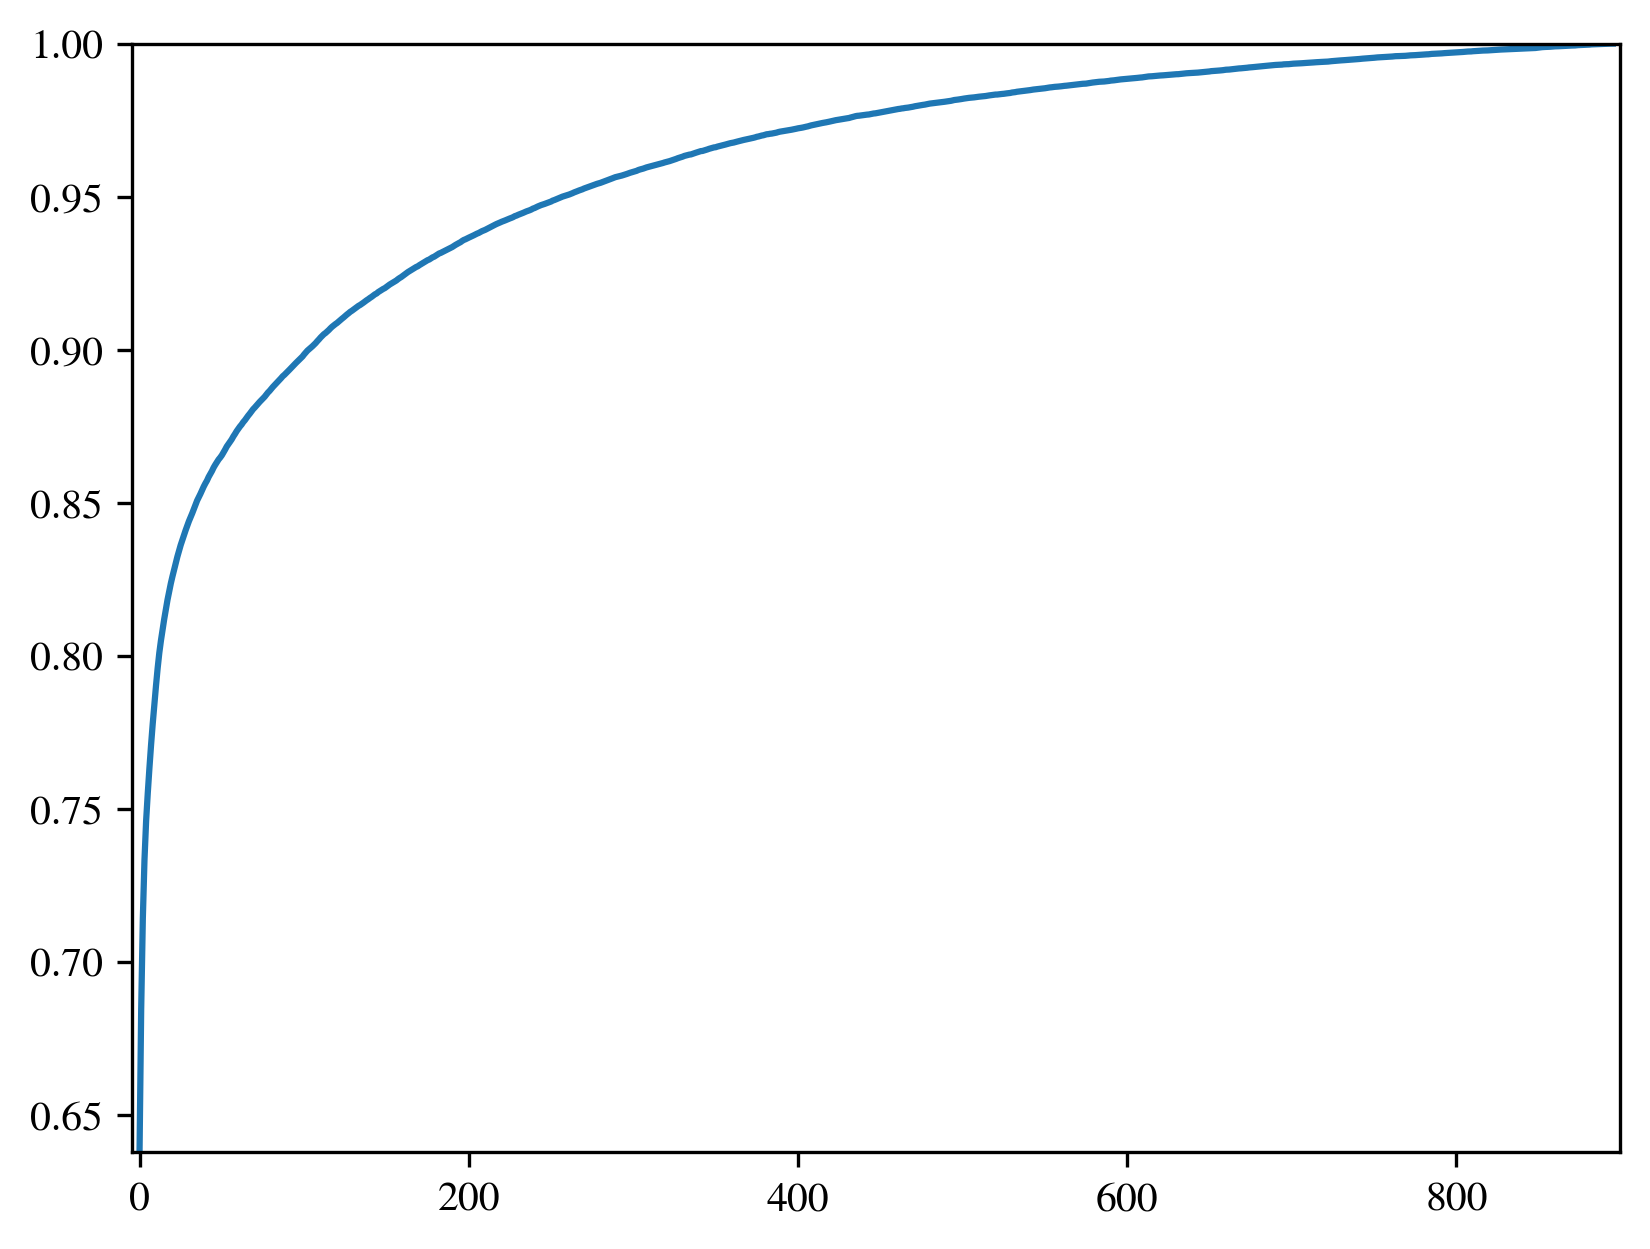
\includegraphics[width=0.4\textwidth]{figures/cdf.png}
%    \caption{
%        The cumulative distribution function of the times when new seeds 
%        were discovered during \stagetwo. 95\% of seeds are found before 7 minutes.
%    }
%    \label{fig:cdf}
%\end{figure}
%
%\begin{figure}[H]
%    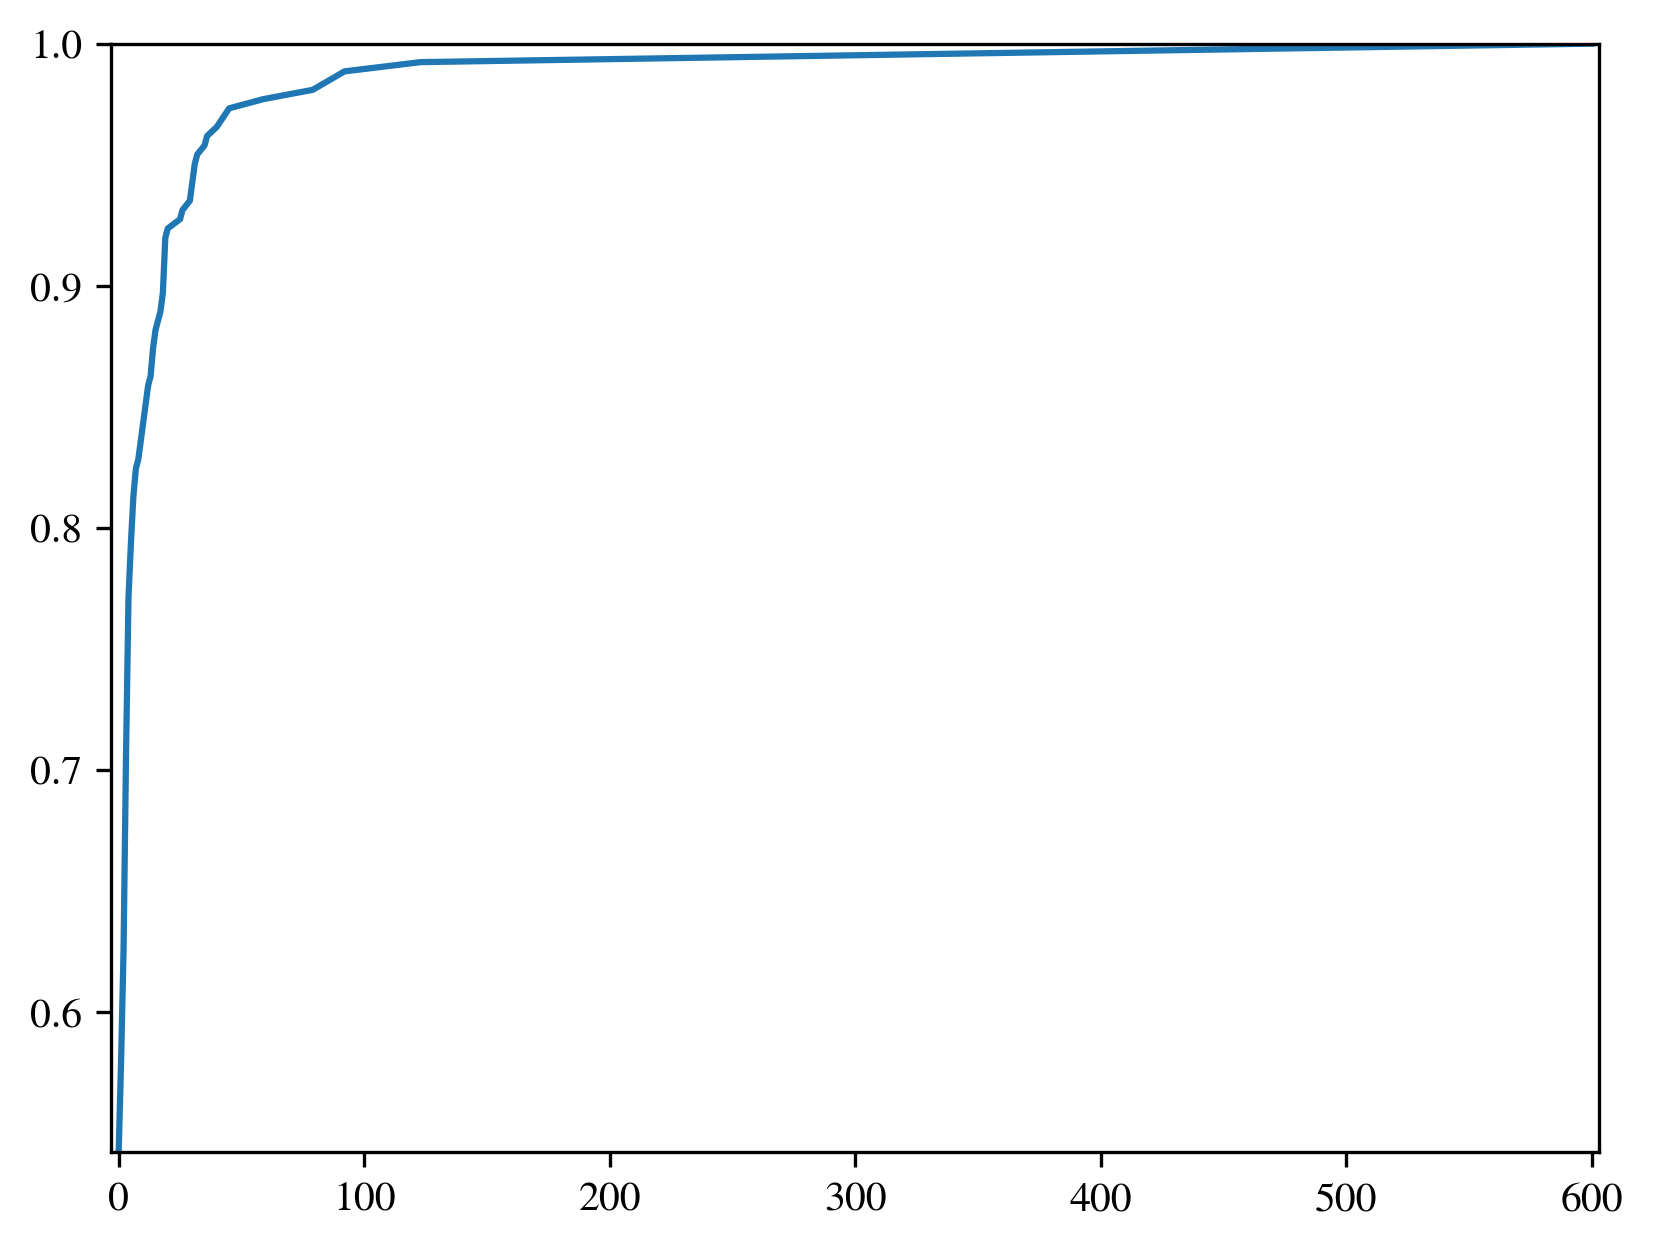
\includegraphics[width=0.4\textwidth]{figures/cdfcrashes.png}
%    \caption{
%        The cumulative distribution function of the times when new crashes 
%        were discovered during \stagetwo. 90\% of crashes are found before 1 minute.
%    }
%    \label{fig:cdfcrashes}
%\end{figure}

%%%%%%%%%%%%%%%%%%%%%%%%%%%%%%%%%%%%%%%%%%%%%%%%%%%%%%%%%%%%%%%%%%%%%%%%%%%%%%%%
\end{document}
%%%%%%%%%%%%%%%%%%%%%%%%%%%%%%%%%%%%%%%%%%%%%%%%%%%%%%%%%%%%%%%%%%%%%%%%%%%%%%%%
